\documentclass{bts-report}

%% ============================================================
%% METADATA CONFIGURATION
%% ============================================================
\theme{Conception et R\'ealisation d'une Application Web de Gestion de la Calibration des \'Equipements de Mesure et de M\'etrologie Industrielle}
\hostorg{Laboratoire National d'\'Etalonnage et de M\'etrologie Industrielle (LNEMI)}
\supervisor{Mme Benayache Samira}
\promoter{M. Samir Mohalbi}
\students{Bassem [Nom de l'\'Etudiant] \\ {[Bin\^ome de Projet]}}
\promotion{2024 / 2026}

\begin{document}

%% ============================================================
%% PAGE DE GARDE OFFICIELLE
%% ============================================================
\maketitlepage

%% ============================================================
%% FRONT MATTER (Num\'erotation romaine)
%% ============================================================
\frontmatter

%% ------------------------------------------------------------
%% REMERCIEMENTS
%% ------------------------------------------------------------
\begin{remerciements}
Avant tout, nous tenons \`a remercier Dieu le Tout-Puissant qui nous a donn\'e la force, le courage, la sant\'e et la volont\'e d'accomplir ce modeste travail et de mener \`a bien cette formation d'avenir.

Nous exprimons notre profonde gratitude et nos sinc\`eres remerciements \`a notre encadreur acad\'emique, \textbf{Mme Benayache Samira}, pour son soutien inestimable, ses orientations p\'edagogiques \'eclair\'ees et ses pr\'ecieux conseils tout au long de la r\'ealisation de ce projet.

Nos vifs remerciements s'adressent \'egalement \`a notre promoteur en entreprise, \textbf{M. Samir Mohalbi}, pour sa disponibilit\'e constante, son encadrement m\'ethodologique rigoureux et son expertise industrielle sans faille.

Nous tenons aussi \`a t\'emoigner toute notre consid\'eration aux membres du jury qui nous font l'honneur d'\'evaluer notre travail, ainsi qu'\`a l'ensemble du corps professoral et administratif de l'\textbf{Institut National Sp\'ecialis\'e de Formation Professionnelle (INSFP) Rahmania - Sidi Abdellah}, pour la qualit\'e de l'enseignement dispens\'e durant notre cursus de Technicien Sup\'erieur.

Enfin, nous adressons un hommage chaleureux \`a tous nos camarades de promotion et \`a toutes les personnes qui ont contribu\'e de pr\`es ou de loin \`a l'aboutissement de cette oeuvre.
\end{remerciements}

%% ------------------------------------------------------------
%% D\'EDICACES
%% ------------------------------------------------------------
\begin{dedicace}
\begin{center}
\vspace*{2cm}
{\itshape
Du plus profond de mon coeur, je d\'edie ce modeste travail :

\`A ma tr\`es ch\`ere m\`ere, source d'amour, de tendresse et de bienveillance, qui a veill\'e sur mes pas avec ses pri\`eres b\'enies tout au long de ma vie.

\`A la m\'emoire de mon cher p\`ere, que Dieu l'accueille dans son vaste paradis, qui m'a appris la pers\'ev\'erance, l'int\'egrit\'e et la valeur de l'effort, et dont le souvenir ne me quitte jamais.

\`A mes tr\`es chers fr\`eres et soeurs, pour leur affection ind\'efectible, leur encouragement constant et leur pr\'esence \`a chaque \'etape de mon parcours.

\`A toute ma famille et mes proches, pour leur soutien moral et leur bienveillance.

\`A tous mes amis fid\`eles et compagnons d'\'etude avec qui j'ai partag\'e des moments inoubliables.

\`A tous ceux qui aiment le savoir et l'excellence.
}
\end{center}
\end{dedicace}

%% ------------------------------------------------------------
%% R\'ESUM\'E FRANCAIS
%% ------------------------------------------------------------
\begin{abstractfr}
La m\'etrologie industrielle et l'\'etalonnage p\'eriodique des \'equipements de mesure constituent un pilier strat\'egique incontournable pour garantir la conformit\'e aux normes de qualit\'e internationales (ISO/IEC 17025) et pr\'evenir les d\'efaillances dans les cha\^ines de production. 

Ce m\'emoire pr\'esente la conception et la r\'ealisation d'une application web d'entreprise d\'edi\'ee \`a la gestion int\'egrale du cycle de vie des op\'erations de calibration couvrant six domaines physiques majeurs (pression, temp\'erature, \'electricit\'e, dimensionnel, pesage et couple). La solution r\'eunit sur une plateforme unique les clients industriels, le service commercial, le responsable m\'etrologie et les techniciens de laboratoire. D\'evelopp\'ee avec une architecture moderne reposant sur \textbf{Laravel}, \textbf{Inertia.js}, \textbf{React 19}, \textbf{TypeScript} et \textbf{MySQL}, l'application int\`egre un contr\^ole d'acc\`es strict bas\'e sur les r\^oles (RBAC), une isolation \'etanche des donn\'ees clients, l'immutabilit\'e des certificats d'\'etalonnage d\'efinitifs, la gestion des \'etalons de r\'ef\'erence et une piste d'audit inalt\'erable. Une suite de 67 tests automatis\'es valide la robustesse et la conformit\'e du syst\`eme.

\vspace{0.6cm}
\noindent\textbf{Mots-cl\'es :} Calibration d'\'equipements, M\'etrologie industrielle, Laravel, Inertia.js, React, Certificats officiels, Immutabilit\'e, Piste d'audit, Norme ISO 17025.
\end{abstractfr}

%% ------------------------------------------------------------
%% ABSTRACT ENGLISH
%% ------------------------------------------------------------
\begin{abstracten}
Industrial metrology and periodic equipment calibration represent a vital foundation for ensuring precision manufacturing, operational safety, and compliance with international quality standards such as ISO/IEC 17025. 

This thesis presents the comprehensive design and engineering of an enterprise web platform managing the end-to-end lifecycle of measurement equipment calibration across six physical domains (pressure, temperature, electrical, dimensional, mass, and torque). The application connects industrial clients, commercial representatives, metrology managers, and qualified calibration technicians within a single unified workspace. Built upon a high-performance architectural stack combining \textbf{Laravel}, \textbf{Inertia.js}, \textbf{React 19}, \textbf{TypeScript}, and \textbf{MySQL}, the system enforces role-based authorization (RBAC), multi-tenant client isolation, strict immutability of finalized calibration certificates, automated reference standards expiration alerts, and comprehensive audit trail logging. The platform is verified through an automated suite of 67 feature tests achieving 100\% passing coverage.

\vspace{0.6cm}
\noindent\textbf{Keywords :} Equipment Calibration, Industrial Metrology, Laravel, Inertia.js, React, Digital Certificates, Immutability, Audit Trail, ISO 17025.
\end{abstracten}

%% ------------------------------------------------------------
%% ABSTRACT ARABIC
%% ------------------------------------------------------------
\begin{abstractar}
تعتبر المترولوجيا الصناعية والمعايرة الدورية لمعدات وأدوات القياس من الركائز الاستراتيجية الأساسية لضمان جودة المنتجات، ودقة التصنيع، وتحقيق مطابقة المعايير الدولية (ISO/IEC 17025). 

يقدم هذا العمل تصميم وإنجاز تطبيق ويب متكامل ومخصص لتسيير دورة الحياة الشاملة لعمليات معايرة وتدقيق الأجهزة القياسية عبر ستة مجالات فيزيائية رئيسية (الضغط، الحرارة، الكهرباء، الأبعاد، الوزن والكتلة، وعزم الدوران). تسمح هذه المنصة بالربط الفعال والمباشر بين الزبائن من المؤسسات الصناعية، المصلحة التجارية، مسؤولي مخبر المترولوجيا، والتقنيين المؤهلين لتنفيذ التجارب. 

تم تطوير النظام وفق معمارية برمجية حديثة تعتمد على إطار العمل \textbf{Laravel} مع تقنية \textbf{Inertia.js} ومكتبة \textbf{React 19} ولغة \textbf{TypeScript}، وقاعدة بيانات \textbf{MySQL}، مع إدماج نظام صلاحيات محكم (RBAC)، وعزل كامل لبيانات الزبائن، وضمان عدم قابلية تعديل شهادات المعايرة النهائية، ومتابعة آلية لصلاحية العتاد المرجعي، وسجل تدقيق أمني شامل لكافة العمليات. تم تأكيد موثوقية التطبيق من خلال 67 اختباراً مؤتمتاً بنجاح تام.

\vspace{0.6cm}
\noindent\textbf{الكلمات المفتاحية :} معايرة المعدات، مترولوجيا صناعية، Laravel، React، Inertia.js، شهادات المعايرة، الأمان الرقمي، تدقيق العمليات.
\end{abstractar}

%% ------------------------------------------------------------
%% SOMMAIRE & LISTES
%% ------------------------------------------------------------
\tableofcontents
\listoffigures
\listoftables

%% ------------------------------------------------------------
%% TABLE DES ABR\'EVIATIONS
%% ------------------------------------------------------------
\abbreviations{
\begin{abbrevtable}
  \ucfield{BTS}{Brevet de Technicien Sup\'erieur}
  \ucfield{INSFP}{Institut National Sp\'ecialis\'e de Formation Professionnelle}
  \ucfield{LNEMI}{Laboratoire National d'\'Etalonnage et de M\'etrologie Industrielle}
  \ucfield{ISO}{International Organization for Standardization}
  \ucfield{IEC}{International Electrotechnical Commission}
  \ucfield{UML}{Unified Modeling Language}
  \ucfield{UP}{Unified Process (M\'ethode Unifi\'ee)}
  \ucfield{MVC}{Mod\`ele - Vue - Contr\^oleur}
  \ucfield{SPA}{Single Page Application}
  \ucfield{API}{Application Programming Interface}
  \ucfield{RBAC}{Role-Based Access Control}
  \ucfield{ORM}{Object-Relational Mapping}
  \ucfield{LEMP}{Linux, Nginx, MySQL, PHP}
  \ucfield{CSRF}{Cross-Site Request Forgery}
  \ucfield{XSS}{Cross-Site Scripting}
  \ucfield{SGBD}{Syst\`eme de Gestion de Base de Donn\'ees}
  \ucfield{ACID}{Atomicit\'e, Coh\'erence, Isolation, Durabilit\'e}
  \ucfield{NIF}{Num\'ero d'Identification Fiscale}
  \ucfield{TVA}{Taxe sur la Valeur Ajout\'ee}
  \ucfield{HTTP}{HyperText Transfer Protocol}
  \ucfield{HTTPS}{HyperText Transfer Protocol Secure}
  \ucfield{SSL/TLS}{Secure Sockets Layer / Transport Layer Security}
\end{abbrevtable}
}

%% ============================================================
%% MAIN MATTER (Num\'erotation arabe d\`es l'Introduction)
%% ============================================================
\mainmatter

%% ============================================================
%% INTRODUCTION G\'EN\'ERALE
%% ============================================================
\chapter*{Introduction G\'en\'erale}
\addcontentsline{toc}{chapter}{Introduction G\'en\'erale}

\section*{1. Contexte G\'en\'eral (\arabtext{السياق العام})}
Dans le contexte de mutation technologique et d'expansion industrielle rapide que conna\^it le secteur manufacturier et \'energ\'etique, la ma\^itrise de la pr\'ecision de mesure repr\'esente un imp\'eratif absolu. Qu'il s'agisse de contr\^oler la pression au sein d'une conduite de gaz, de mesurer des temp\'eratures critiques dans des r\'eacteurs chimiques ou de v\'erifier les tol\'erances biom\'ecaniques et dimensionnelles de pi\`eces d'usinage, chaque d\'ecision industrielle repose sur la fiabilit\'e d'un instrument de mesure. La m\'etrologie industrielle, r\'egie par des r\'ef\'erentiels rigoureux tels que la norme internationale \textbf{ISO/IEC 17025}, impose que tout \'equipement soit raccord\'e aux \'etalons nationaux et v\'erifi\'e selon des cycles de calibration d\'etermin\'es.

Parall\`element, la transformation num\'erique des entreprises est devenue le levier fondamental pour optimiser l'efficacit\'e op\'erationnelle, r\'eduire les d\'elais de traitement et garantir une tra\^itabilit\'e infaillible des donn\'ees. L'abandon progressif des fiches manuelles et des registres d'atelier au profit de syst\`emes d'information web centralis\'es offre aux organisations une r\'eactivit\'e sup\'erieure, un archivage s\'ecuris\'e et une communication fluide entre les diff\'erents acteurs de la cha\^ine de valeur.

C'est dans cette optique que s'inscrit notre projet de fin d'\'etudes, portant sur la conception et la r\'ealisation d'une application web d'entreprise de gestion compl\`ete du cycle de vie de la calibration des \'equipements au profit d'un laboratoire de m\'etrologie industrielle.

\section*{2. Probl\'ematique et Hypoth\`ese de Travail (\arabtext{الإشكالية وفرضية العمل})}
Malgr\'e l'importance critique de la calibration, de nombreux laboratoires et services de maintenance op\`erent encore selon des proc\'edures semi-manuelles fragment\'ees, caract\'eris\'ees par l'utilisation de tableurs \'eparpill\'es, de courriers \'electroniques non trac\'es et de documents papier physiques. Cette situation engendre plusieurs probl\`emes majeurs :
\begin{itemize}
  \item \textbf{Lenteur du traitement administratif :} D\'elais importants entre la soumission d'une demande par le client, son examen commercial, la planification de l'intervention et l'\'emission des devis.
  \item \textbf{Risque m\'etrologique majeur :} L'absence de contr\^ole automatis\'e peut conduire \`a l'utilisation involontaire d'\'etalons de r\'ef\'erence p\'erim\'es, compromettant la validit\'e l\'egale des r\'esultats de mesure.
  \item \textbf{D\'eficit de tra\^itabilit\'e et risque de falsification :} Les rapports d'essais physiques \'echangent de main en main sans journalisation pr\'ecise des modifications, et les certificats \'emis sur papier peuvent \^etre alt\'er\'es.
  \item \textbf{Insatisfaction du client industriel :} Impossibilit\'e pour les clients de suivre en temps r\'eel l'avancement de leurs dossiers et lenteur d'acc\`es aux certificats n\'ecessaires aux audits de conformit\'e.
\end{itemize}

D\`es lors, la probl\'ematique centrale de notre travail s'\'enonce ainsi :
\begin{quote}
\itshape
\og Comment concevoir et d\'evelopper une plateforme web hautement s\'ecuris\'ee, modulaire et r\'eactive, capable d'automatiser et d'encadrer rigoureusement l'int\'egralit\'e du cycle de vie des op\'erations de calibration d'\'equipements, tout en garantissant l'isolation des donn\'ees clients, l'immutabilit\'e des certificats et une tra\^itabilit\'e d'audit totale ? \fg
\end{quote}

Notre hypoth\`ese de travail repose sur le fait qu'une architecture web moderne \`a trois niveaux, associant la robustesse transactionnelle de \textbf{Laravel 12} et l'ergonomie dynamique de \textbf{React 19} via \textbf{Inertia.js}, combin\'ee \`a un moteur d'habilitations strict (RBAC) et un verrouillage d'immutabilit\'e au niveau des certificats finaux, permettra de fluidifier les processus m\'etrologiques, d'\'eliminer les erreurs de saisie et de fournir aux industriels des preuves m\'etrologiques certifi\'ees conformes.

\section*{3. Objectifs du Projet (\arabtext{أهداف المشروع})}
Pour r\'epondre \`a cette probl\'ematique, les objectifs strat\'egiques et op\'erationnels fix\'es sont :
\begin{enumerate}
  \item Mettre \`a disposition un portail client s\'ecuris\'e permettant la consultation du catalogue m\'etrologique (6 domaines) et la cr\'eation de demandes d'\'etalonnage multi-\'equipements en une seule transaction.
  \item Structurer le traitement commercial par la qualification des demandes et la g\'en\'eration automatis\'ee de devis chiffr\'es avec calcul des taxes l\'egales (HT, TVA 19\%, TTC).
  \item Mettre en place un processus de n\'egociation et de concertation des dates et lieux d'intervention (en laboratoire ou sur site industriel).
  \item Assurer l'affectation \'equilibr\'ee des op\'erations aux techniciens m\'etrologues qualifi\'es avec gestion des revues qualit\'e et des reprises techniques (\textit{rework}).
  \item Garantir la conformit\'e l\'egale par la production de certificats d'\'etalonnage initialis\'es en brouillon puis scell\'es d'un verrou d'immutabilit\'e d\'efinitif (\texttt{is\_final = true}) avec support de d\'el\'egation trac\'ee de signature.
  \item Centraliser la surveillance des \'etalons de r\'ef\'erence avec d\'etection et blocage automatique des instruments dont la validit\'e m\'etrologique est expir\'ee.
  \item \'Etablir une piste d'audit inalt\'erable enregistrant chaque \'ev\'enement sensible (acteur, date, adresse IP, anciennes et nouvelles valeurs).
\end{enumerate}

\section*{4. Structure de la M\'emoire (\arabtext{خطة المذكرة})}
Conform\'ement aux directives acad\'emiques de l'INSFP Rahmania et aux mod\`eles de r\'ef\'erence, notre m\'emoire est structur\'e en quatre chapitres compl\'ementaires :
\begin{itemize}
  \item \textbf{Chapitre I : Notions G\'en\'erales et Fondements Th\'eoriques :} D\'edi\'e \`a l'\'etat de l'art des technologies web, \`a l'architecture client-serveur, aux protocoles de communication, aux frameworks utilis\'es (Laravel, Inertia, React) et aux principes de s\'ecurit\'e applicative.
  \item \textbf{Chapitre II : \'Etude Pr\'ealable et Pr\'esentation de l'Organisme d'Accueil :} Consacr\'e \`a la pr\'esentation du laboratoire d'\'etalonnage, \`a son organigramme, \`a l'analyse critique de l'existant, aux sp\'ecifications des besoins et \`a la d\'emarche m\'ethodologique.
  \item \textbf{Chapitre III : Analyse et Conception Syst\`eme :} D\'eveloppe la mod\'elisation conceptuelle et d\'etaill\'ee \`a l'aide d'UML (cas d'utilisation, fiches descriptives, s\'equences chronologiques, machine \`a \'etats, classes du domaine, dictionnaire de donn\'ees et d\'eploiement).
  \item \textbf{Chapitre IV : R\'ealisation, Interfaces et Validation :} Expose l'environnement de d\'eveloppement, l'architecture logicielle, les maquettes des \'ecrans r\'ealis\'es, ainsi que la strat\'egie et les m\'etriques de tests automatis\'es validant le syst\`eme.
\end{itemize}

Le m\'emoire se cl\^oture par une conclusion g\'en\'erale dressant le bilan des r\'esultats obtenus et tra\c{c}ant les perspectives d'\'evolution futures du projet.


%% ============================================================
%% CHAPITRE I : FONDEMENTS TH\'EORIQUES
%% ============================================================
\chapter{Notions G\'en\'erales et Fondements Th\'eoriques}

\section*{Introduction du Chapitre}
L'\'elaboration d'une application d'entreprise moderne n\'ecessite une compr\'ehension approfondie des fondements th\'eoriques du d\'eveloppement logiciel, des mod\`eles architecturaux contemporains et des technologies d'ing\'enierie du Web. Ce premier chapitre \'etablit le cadre conceptuel de notre projet. Nous y \'etudions les r\'eseaux informatiques et l'architecture client-serveur, avant de d\'etailler l'\'ecosyst\`eme technologique retenu pour la couche cliente (React, TypeScript, Tailwind CSS) et la couche serveur (Laravel, PHP, MySQL), en mettant un accent particulier sur le pont r\'eactif Inertia.js et les paradigmes de s\'ecurit\'e applicative.

\section{R\'eseaux et Concepts Fondamentaux du Web}
\subsection{D\'efinition d'Internet et du Web}
Bien que fr\'equemment employ\'es de mani\`ere interchangeable dans le langage courant, les termes \textit{Internet} et \textit{Web} recouvrent deux r\'ealit\'es techniques distinctes mais \'etroitement interd\'ependantes :
\begin{itemize}
  \item \textbf{Internet :} Repr\'esente l'infrastructure r\'eseau mondiale maill\'ee reliant des centaines de millions d'\'equipements informatiques. Elle op\`ere gr\^ace \`a une suite standardis\'ee de protocoles d\'enomm\'ee \textbf{TCP/IP} (Transmission Control Protocol / Internet Protocol), assurant l'adressage num\'erique des h\^otes et le routage des paquets de donn\'ees \`a l'\'echelle plan\'etaire.
  \item \textbf{Le Web (World Wide Web) :} Constitue un syst\`eme d'information hyperm\'edia distribu\'e qui fonctionne au-dessus de l'infrastructure Internet. Con\c{c}u initialement par Tim Berners-Lee au CERN en 1989, le Web permet de consulter et d'interconnecter des ressources multim\'edias (textes, images, vid\'eos) au moyen d'adresses universelles (URI/URL) et du protocole de transfert hypertexte.
\end{itemize}

\subsection{Protocoles de Communication HTTP et HTTPS}
Le protocole \textbf{HTTP} (HyperText Transfer Protocol) est un protocole de la couche application, stateless (sans \'etat) et fonctionnant selon un mod\`ele requ\^ete-r\'eponse. Chaque interaction d\'ebute par l'\'emission d'une requ\^ete client comportant une m\'ethode sp\'ecifique (GET pour la lecture, POST pour la cr\'eation, PUT/PATCH pour la mise \`a jour, DELETE pour la suppression), des en-t\^etes de m\'etadonn\'ees et \'eventuellement un corps (\textit{body}) contenant des donn\'ees encod\'ees (JSON, formulaires multipart).

Dans les applications manipulant des donn\'ees m\'etrologiques sensibles, l'usage de \textbf{HTTPS} (HTTP Secure) est imp\'eratif. HTTPS encapsule les flux HTTP dans un canal chiffr\'e par le protocole cryptographique \textbf{TLS} (Transport Layer Security, version 1.3), garantissant trois piliers fondamentaux :
\begin{enumerate}
  \item \textbf{La confidentialit\'e :} Aucun tiers espion sur le r\'eseau ne peut intercepter les identifiants ou les devis financiers en clair.
  \item \textbf{L'int\'egrit\'e :} Les paquets transmis ne peuvent \^etre alt\'er\'es ou falsifi\'es durant le transit.
  \item \textbf{L'authentification du serveur :} Le certificat num\'erique X.509 d\'elivr\'e par une autorit\'e de certification valide l'identit\'e l\'egitime du laboratoire.
\end{enumerate}

\section{Architecture Client-Serveur et Paradigmes Modernes}
\subsection{Le Mod\`ele 3-Tiers}
Notre plateforme s'appuie sur une architecture d\'ecoup\'ee en trois tiers logiques ind\'ependants, offrant une haute maintenabilit\'e, une mont\'ee en charge ma\^itris\'ee et une stricte s\'eparation des responsabilit\'es :
\begin{enumerate}
  \item \textbf{Le Tiers Pr\'esentation (Client) :} Ex\'ecut\'e au sein du navigateur de l'utilisateur. Il re\c{c}oit les donn\'ees au format structur\'e JSON et assure le rendu dynamique des composants d'interface, la gestion des \'etats locaux et la capture des \'ev\'enements utilisateurs.
  \item \textbf{Le Tiers Traitement (Serveur d'Application) :} H\'eberg\'e sur le serveur d'entreprise. Il impl\'emente la logique m\'etier m\'etrologique, orchestre les transactions, applique les r\`egles d'habilitation et traite les flux d'approbation.
  \item \textbf{Le Tiers Donn\'ees (SGBD) :} D\'edi\'e au stockage p\'erenne, \`a l'indexation et \`a la restitution transactionnelle des donn\'ees via le moteur relationnel MySQL.
\end{enumerate}

\begin{figure}[H]
  \centering
  \begin{tikzpicture}[>=stealth, node distance=1.5cm and 2cm,
    tier/.style={draw=blue!70!black, fill=blue!5, rounded corners=4pt, line width=1pt, minimum width=3.2cm, minimum height=1.6cm, align=center, font=\small},
    db/.style={draw=orange!80!black, fill=orange!10, rounded corners=4pt, line width=1pt, minimum width=3.2cm, minimum height=1.6cm, align=center, font=\small},
    arrow/.style={->, thick, >=stealth, color=darkgray}
]
\node[tier] (client) {\textbf{Tier 1 : Client}\\[2pt]Navigateur Web / Client\\React 19 + TypeScript\\Tailwind CSS v4};
\node[tier, right=2.2cm of client] (server) {\textbf{Tier 2 : Serveur}\\[2pt]Serveur Web \& API\\Laravel 12/13 (PHP 8.2+)\\Inertia.js + Auth RBAC};
\node[db, right=2.2cm of server] (database) {\textbf{Tier 3 : Donn\'ees}\\[2pt]Syst\`eme SGBD\\MySQL 8.0+ / Eloquent\\Int\'egrit\'e ACID \& Audit};

\draw[arrow] (client.north east) -- node[above, font=\footnotesize, align=center] {Requ\^etes HTTPS / JSON\\(Inertia Visits)} (server.north west);
\draw[arrow] (server.south west) -- node[below, font=\footnotesize, align=center] {Props JSON \& Vues\\Rendu R\'eactif} (client.south east);

\draw[arrow] (server.north east) -- node[above, font=\footnotesize, align=center] {Requ\^etes SQL\\ORM Eloquent} (database.north west);
\draw[arrow] (database.south west) -- node[below, font=\footnotesize, align=center] {R\'esultats \& Curseurs\\Transactions} (server.south east);
\end{tikzpicture}

  \caption{Architecture Client-Serveur 3-Tiers de la Plateforme M\'etrologique}
  \label{fig:web-arch}
\end{figure}

\subsection{Le Paradigme Hybride Inertia.js}
Traditionnellement, les ing\'enieurs web devaient choisir entre deux extr\^emes architecturaux :
\begin{itemize}
  \item Les applications monolithiques classiques avec rendu c\^ot\'e serveur (\textit{Server-Side Rendering}), robustes mais entra\^inant des rechargements complets de page peu ergonomiques ;
  \item Les applications monopages (\textit{Single Page Applications} - SPA) d\'ecoupl\'ees, fluides mais n\'ecessitant la construction d'une API REST distincte, la duplication des validations et la gestion complexe des tokens JWT d'authentification.
\end{itemize}

\textbf{Inertia.js} constitue une rupture m\'ethodologique \'el\'egante en agissant comme une \og passerelle r\'eactive \fg. Gr\^ace au protocole HTTP d'en-t\^etes \texttt{X-Inertia}, il permet de conserver le mod\`ele de contr\^oleur et de routage centralis\'e c\^ot\'e serveur de Laravel, tout en confiant l'int\'egralit\'e du rendu visuel aux composants React c\^ot\'e client, sans rupture de page.

\begin{figure}[H]
  \centering
  \begin{tikzpicture}[>=Stealth,
    block/.style={draw=blue!70!black, fill=blue!15, rounded corners=3pt, line width=0.8pt, minimum width=4.0cm, minimum height=1.6cm, align=center, font=\footnotesize},
    bridge/.style={draw=orange!80!black, fill=orange!10, rounded corners=3pt, line width=0.8pt, minimum width=4.0cm, minimum height=1.6cm, align=center, font=\footnotesize},
    backend/.style={draw=blue!70!black, fill=blue!5, rounded corners=3pt, line width=0.8pt, minimum width=4.0cm, minimum height=1.6cm, align=center, font=\footnotesize},
    arrow/.style={->, line width=0.8pt, >=Stealth, color=darkgray}
]
\node[block] (react) {\textbf{Frontend React 19}\\[2pt]Composants UI / Pages\\State Management};
\node[bridge, right=2.6cm of react] (inertia) {\textbf{Passerelle Inertia.js}\\[2pt]Protocole X-Inertia\\Routage Hybride Monolithique};
\node[backend, right=2.6cm of inertia] (laravel) {\textbf{Backend Laravel 12}\\[2pt]Contr\^oleurs / Middleware\\Mod\`eles Eloquent};

\draw[arrow] (react.east) -- node[above, font=\footnotesize] {Inertia.visit()} (inertia.west);
\draw[arrow] (inertia.east) -- node[above, font=\footnotesize] {Route / Action} (laravel.west);
\draw[arrow] ([yshift=-0.35cm]laravel.south west) to[bend left=35] node[below, font=\footnotesize] {Inertia::render('Page', \$props)} ([yshift=-0.35cm]react.south east);
\end{tikzpicture}
  \caption{Mod\`ele de Communication R\'eactif via la Passerelle Inertia.js}
  \label{fig:inertia-bridge}
\end{figure}

\section{Technologies et Outils C\^ot\'e Client (Frontend)}
\subsection{React 19 et Approche par Composants}
\textbf{React 19} est une biblioth\`eque JavaScript d\'evelopp\'ee par Meta, con\c{c}ue pour b\^atir des interfaces utilisateur r\'eactives et modulaires. Son architecture repose sur la d\'ecomposition de l'\'ecran en composants r\'eutilisables et autonomes (ex. : s\'electeur d'\'equipement, badge de statut, tableau d'audit). React optimise les performances gr\^ace \`a son \textit{Virtual DOM}, qui calcule les diff\'erences algorithmiques et n'applique au DOM r\'eel que les modifications strictes n\'ecessaires.

\subsection{TypeScript pour la Fiabilit\'e du Code}
\textbf{TypeScript}, sur-ensemble typ\'e de JavaScript cr\'e\'e par Microsoft, ajoute un syst\`eme de typage statique rigoureux. Dans une application m\'etrologique o\`u chaque \'equipement poss\`ede des attributs stricts (num\'ero de s\'erie, \'etendue de mesure, tol\'erance), TypeScript permet de d\'efinir des interfaces de donn\'ees explicites (\texttt{interface CalibrationRequest}, \texttt{interface EquipmentItem}). Les erreurs de frappe ou de types sont d\'etect\'ees d\`es la compilation, garantissant un code d\'enue de r\'egressions.

\subsection{Tailwind CSS v4 et Vite}
\textbf{Tailwind CSS v4} est un framework CSS utilitaire moderne qui permet de styliser les composants directement au moyen de classes atomiques optimis\'ees. Son compilateur natif analyse le code source et ne conserve en production que les r\`egles CSS r\'eellement utilis\'ees, assurant une l\'eg\`eret\'e maximale des pages.

L'ensemble de la cha\^ine de compilation c\^ot\'e client est pilot\'e par \textbf{Vite 8}, un outillage de nouvelle g\'en\'eration propuls\'e par Rollup et le protocole natif ES Modules, offrant un rechargement \`a chaud instantan\'e (\textit{Hot Module Replacement} - HMR) lors du d\'eveloppement.

\section{Technologies et Outils C\^ot\'e Serveur (Backend)}
\subsection{Langage PHP 8.2+ et Architecture MVC}
\textbf{PHP} demeure l'un des piliers du Web mondial. Ses versions r\'ecentes (8.2+) introduisent des avanc\'ees majeures en termes de performances et de rigueur formelle : compilation JIT (\textit{Just-In-Time}), typage strict des propri\'et\'es, \'enum\'erations natives et gestion optimis\'ee de la m\'emoire. Le mod\`ele architectural \textbf{MVC} (Mod\`ele - Vue - Contr\^oleur) assure une s\'eparation nette :
\begin{itemize}
  \item \textbf{Le Mod\`ele :} Repr\'esente les donn\'ees et les r\`egles m\'etier (ex. : validation de date, calcul des taxes).
  \item \textbf{La Vue :} Assure la restitution visuelle (confi\'ee \`a React via Inertia).
  \item \textbf{Le Contr\^oleur :} R\'eceptionne les requ\^etes HTTP, orchestre l'appel aux mod\`eles et d\'el\`egue l'affichage.
\end{itemize}

\subsection{Le Framework Laravel 12/13 et Eloquent ORM}
\textbf{Laravel} est le framework PHP de r\'ef\'erence mondial. Il int\`egre un ensemble complet d'outils d'entreprise :
\begin{itemize}
  \item \textbf{Eloquent ORM :} Un mappeur objet-relationnel tr\`es expressif bas\'e sur le patron \textit{Active Record}, permettant de manipuler les tables sous forme d'objets m\'etier et de d\'efinir les relations (\texttt{hasMany}, \texttt{belongsTo}, \texttt{belongsToMany}).
  \item \textbf{Migrations et Seeders :} Gestion du sch\'ema de base de donn\'ees sous contr\^ole de version et g\'en\'eration de jeux d'essais coh\'erents.
  \item \textbf{Middleware et Policies :} Filtrage des requ\^etes en amont des contr\^oleurs pour valider les jetons CSRF et contr\^oler les autorisations d'acc\`es.
\end{itemize}

\subsection{Le SGBD Relationnel MySQL}
Pour assurer la persistance, notre choix s'est port\'e sur \textbf{MySQL 8.0+}. Reconnu pour sa rapidit\'e et son impl\'ementation stricte des propri\'et\'es \textbf{ACID}, MySQL garantit que chaque cr\'eation de demande multi-\'equipements s'ex\'ecute au sein d'une transaction atomique : si l'un des enregistrements \'echoue, l'int\'egralit\'e de l'op\'eration est annul\'ee (\textit{rollback}), \'evitant toute corruption ou orphelinat de donn\'ees.

\section{S\'ecurit\'e et Mod\`ele d'Habilitation (RBAC)}
La s\'ecurit\'e d'une application m\'etrologique industrielle est vitale. Notre syst\`eme impl\'emente un contr\^ole d'acc\`es bas\'e sur les r\^oles (\textbf{RBAC} - Role-Based Access Control) :

\begin{figure}[H]
  \centering
  \begin{tikzpicture}[
    >=Stealth,
    line width=0.8pt,
    role/.style={draw=blue!70!black, fill=blue!10, rounded corners=3pt, minimum width=2.8cm, align=center, font=\footnotesize\bfseries},
    perm/.style={draw=gray!60!black, fill=gray!10, rounded corners=3pt, text width=3.2cm, align=center, font=\scriptsize},
    hier/.style={->, >=Stealth, line width=0.8pt},
    permarr/.style={->, >=Stealth, line width=0.8pt, dashed}
]
% --- r\^oles ---
\node[role] (admin) at (0, 0) {Administrateur IT};
\node[role] (manager) at (-4.5, -2.5) {Responsable M\'etrologie};
\node[role] (comm) at (0, -2.5) {Commercial};
\node[role] (tech) at (4.5, -2.5) {Technicien M\'etrologue};
\node[role] (delegate) at (-4.5, -5) {M\'etrologue D\'el\'egu\'e};
\node[role] (client) at (0, -5) {Client Externe};

% --- permissions ---
\node[perm] (p_admin) at (4.5, 0) {G\'erer utilisateurs \textbullet{} R\^oles\\Audit \textbullet{} \'Etalons};
\node[perm] (p_manager) at (-6.5, -7.5) {Affecter \textbullet{} Revue\\Valider certificat};
\node[perm] (p_comm) at (2, -10) {Qualifier \textbullet{} \'Emettre devis\\Contrats};
\node[perm] (p_tech) at (4.5, -7.5) {Prise en charge\\Upload rapports};
\node[perm] (p_delegate) at (-6.5, -10) {Valider certificats\\(Mode d\'el\'egation trac\'e)};
\node[perm] (p_client) at (0, -7.5) {Cr\'eer demandes\\T\'el\'echarger certificats};

% --- hi\'erarchie des r\^oles ---
\draw[hier] (admin.south) |- (manager.north);
\draw[hier] (admin.south) -- (comm.north);
\draw[hier] (admin.south) |- (tech.north);
\draw[hier] (manager.south) -- (delegate.north);

% --- permissions par r\^ole ---
\draw[permarr] (admin.east) -- (p_admin.west);
\draw[permarr] (manager.west) -- (-6.5, -3) -- (p_manager.north);
\draw[permarr] (delegate.south) |- (p_delegate.north);
\draw[permarr] (comm.south) -- (2, -3) -- (p_comm.north);
\draw[permarr] (client.south) -- (p_client.north);
\draw[permarr] (tech.south) -- (p_tech.north);
\end{tikzpicture}
  \caption{Hi\'erarchie des R\^oles et Mod\`ele d'Habilitation (RBAC)}
  \label{fig:rbac-model}
\end{figure}

Le syst\`eme pr\'evient les vuln\'erabilit\'es majeures du Top 10 OWASP :
\begin{itemize}
  \item \textbf{Injections SQL :} Neutralis\'ees gr\^ace \`a l'usage exclusif de requ\^etes param\'etr\'ees dans Eloquent ORM.
  \item \textbf{Attaques CSRF :} Protection automatique via jetons cryptographiques v\'erifi\'es \`a chaque requ\^ete mutatrice (POST/PUT/DELETE).
  \item \textbf{Failles XSS :} \'Echappement contextuel automatique assur\'e par le moteur React.
  \item \textbf{Isolation Multi-Tenants :} Chaque requ\^ete d'un client externe est automatiquement born\'ee par un filtre limitant l'acc\`es \`a son seul identifiant (\texttt{client\_id}).
\end{itemize}

\section*{Conclusion du Chapitre}
Ce premier chapitre a permis de poser les bases th\'eoriques n\'ecessaires \`a la compr\'ehension du projet. L'association de Laravel pour la rigueur transactionnelle du backend et de React/Inertia pour la r\'eactivit\'e du frontend offre une architecture industrielle robuste. Le chapitre suivant pr\'esente l'environnement professionnel de l'organisme d'accueil et d\'eveloppe l'\'etude pr\'ealable de notre solution.


%% ============================================================
%% CHAPITRE II : \'ETUDE PR\'EALABLE
%% ============================================================
\chapter{\'Etude Pr\'ealable et Pr\'esentation de l'Organisme d'Accueil}

\section*{Introduction du Chapitre}
Toute r\'ealisation logicielle r\'eussie prend racine dans une analyse rigoureuse du contexte organisationnel et op\'erationnel dans lequel elle doit s'ins\'erer. Ce deuxi\`eme chapitre est consacr\'e \`a l'\'etude pr\'ealable de notre projet. Nous y pr\'esentons tout d'abord le laboratoire national de m\'etrologie industrielle, son organigramme et ses missions sp\'ecialis\'ees. Nous proc\'edons ensuite \`a un audit m\'ethodique du syst\`eme existant afin d'en d\'egager les limites concr\`etes, avant de formuler les sp\'ecifications d\'etaill\'ees de la solution web propos\'ee et d'exposer la d\'emarche de d\'eveloppement retenue.

\section{Pr\'esentation de l'Organisme d'Accueil}
\subsection{Missions et Vocation Institutionnelle}
Le \textbf{Laboratoire National d'\'Etalonnage et de M\'etrologie Industrielle (LNEMI)} est l'institution de r\'ef\'erence charg\'ee de garantir la tra\^itabilit\'e m\'etrologique des instruments de mesure utilis\'es dans les secteurs \'energetique, p\'etrolier, m\'ecanique, pharmaceutique et agroalimentaire.

Conform\'ement aux exigences de la norme internationale \textbf{ISO/IEC 17025} (Exigences g\'en\'erales concernant la comp\'etence des laboratoires d'\'etalonnages et d'essais), le laboratoire a pour missions principales :
\begin{enumerate}
  \item Assurer le raccordement m\'etrologique des \'etalons industriels aux \'etalons primaires nationaux et internationaux.
  \item R\'ealiser des prestations d'\'etalonnage et de v\'erification en laboratoire accr\'edit\'e ou directement sur les sites industriels clients.
  \item D\'elivrer des certificats officiels d'\'etalonnage et des constats de v\'erification faisant foi aupr\`es des organismes de contr\^ole r\'eglementaires.
  \item Accompagner les entreprises manufacturi\`eres dans l'estimation des incertitudes de mesure et la maintenance de leur parc d'instruments.
\end{enumerate}

\subsection{Domaines M\'etrologiques Couverts}
Le laboratoire d\'eploie ses comp\'etences \`a travers six domaines physiques majeurs :
\begin{itemize}
  \item \textbf{Pression :} \'Etalonnage de manom\`etres industriels, transmetteurs de pression, manom\`etres diff\'erentiels et capteurs pi\'ezo\'electriques (gamme de vide pouss\'e jusqu'\`a 1000 bar).
  \item \textbf{Temp\'erature :} \'Etalonnage de sondes \`a r\'esistance (Pt100), thermocouples industriels et thermom\`etres en bains thermostat\'es ou fours d'\'etalonnage (-50~$^\circ$C \`a 1200~$^\circ$C).
  \item \textbf{Electricit\'e :} \'Etalonnage de multim\`etres de pr\'ecision, pinces amp\`erem\'etriques, r\'esistances \'etalons et oscilloscopes.
  \item \textbf{Dimensionnel :} Contr\^ole m\'etrologique de cales \'etalons, pieds \`a coulisse, microm\`etres et comparateurs de haute pr\'ecision.
  \item \textbf{Pesage et Masse :} V\'erification de masses \'etalons de classe E2 \`a M1 et \'etalonnage de balances d'analyses de laboratoire et de ponts-bascules.
  \item \textbf{Couple :} \'Etalonnage de cl\'es dynamom\'etriques, tournevis dynamom\'etriques et bancs de mesure de torsion.
\end{itemize}

\section{Structure Organisationnelle et Organigramme}
L'organigramme fonctionnel du laboratoire refl\`ete la s\'eparation n\'ecessaire entre les fonctions de gestion commerciale, l'expertise m\'etrologique technique et l'audit qualit\'e ind\'ependant :

\begin{figure}[H]
  \centering
  \begin{tikzpicture}[>=stealth,
    box/.style={draw=black!70, fill=gray!10, rounded corners=3pt, line width=0.8pt, minimum width=3.4cm, minimum height=0.9cm, align=center, font=\footnotesize},
    mainbox/.style={draw=blue!80!black, fill=blue!15, rounded corners=4pt, line width=1.1pt, minimum width=4cm, minimum height=1cm, align=center, font=\small\bfseries},
    arrow/.style={-, thick, color=gray!80}
]
\node[mainbox] (dg) {Direction G\'en\'erale / ALICEF SPA};
\node[box, below=0.9cm of dg, xshift=-4.2cm] (qualite) {\textbf{D\'epartement Qualit\'e}\\[2pt]Norme ISO/IEC 17025};
\node[box, below=0.9cm of dg, xshift=0cm] (technique) {\textbf{Laboratoire M\'etrologie}\\[2pt]Pression, T$^\circ$, \'Elec, Masse};
\node[box, below=0.9cm of dg, xshift=4.2cm] (comm) {\textbf{Service Commercial}\\[2pt]Relation Client \& Devis};

\node[box, below=0.8cm of technique, xshift=-1.8cm] (techniciens) {Techniciens d'\'Etalonnage};
\node[box, below=0.8cm of technique, xshift=1.8cm] (etalons) {Gestionnaire des \'Etalons};

\draw[arrow] (dg.south) -- ++(0,-0.4) -| (qualite.north);
\draw[arrow] (dg.south) -- ++(0,-0.4) -| (technique.north);
\draw[arrow] (dg.south) -- ++(0,-0.4) -| (comm.north);
\draw[arrow] (technique.south) -- ++(0,-0.3) -| (techniciens.north);
\draw[arrow] (technique.south) -- ++(0,-0.3) -| (etalons.north);
\end{tikzpicture}

  \caption{Organigramme Fonctionnel de l'Organisme d'Accueil}
  \label{fig:org-chart}
\end{figure}

\begin{itemize}
  \item \textbf{La Direction G\'en\'erale :} D\'efinit la politique strat\'egique et alloue les ressources mat\'erielles.
  \item \textbf{Le D\'epartement Qualit\'e :} Veille au respect strict du manuel qualit\'e ISO/IEC 17025 et organise les audits p\'eriodiques.
  \item \textbf{Le Laboratoire de M\'etrologie :} Dirig\'e par le Responsable M\'etrologie, qui supervise l'affectation des techniciens et le maintien en conformit\'e des \'etalons de r\'ef\'erence.
  \item \textbf{Le Service Commercial :} Interlocuteur privil\'egi\'e des clients, charg\'e de l'\'emission des devis, de la contractualisation et de la facturation.
\end{itemize}

\section{\'Etude de l'Existant et Critique du Syst\`eme Actuel}
\subsection{Description des Proc\'edures Actuelles}
Dans le fonctionnement actuel, lorsqu'une entreprise industrielle d\'esire faire \'etalonner un lot de manom\`etres ou de sondes, la d\'emarche s'op\`ere \`a travers un circuit hybride papier et courrier \'electronique :
\begin{enumerate}
  \item Le client transmet un listing sommaire par email ou fax au service commercial.
  \item Le commercial cr\'ee manuellement une fiche de dossier sous tableur Excel et la transmet au responsable technique.
  \item La planification de la date d'intervention se n\'egocie par \'echanges t\'el\'ephoniques sans validation \'ecrite formelle.
  \item Le technicien re\c{c}oit une fiche de travail cartonn\'ee, ex\'ecute les mesures et consigne les r\'esultats sur un document manuscrit.
  \item Le responsable m\'etrologie examine la fiche, puis une secr\'etaire saisit le certificat officiel sous traitement de texte Word avant impression et signature manuscrite.
\end{enumerate}

\subsection{Critique du Syst\`eme Existant}
Cette organisation manuelle pr\'esente des faiblesses structurelles majeures :
\begin{itemize}
  \item \textbf{Dispersion des donn\'ees :} Les informations relatives \`a un client sont r\'eparties entre des bo\^ites de messagerie individuelles, des classeurs physiques et des fichiers Excel locaux, cr\'eant des doublons et des incoh\'erences.
  \item \textbf{Lenteur administrative :} Le d\'elai moyen entre la demande initiale et la r\'eception du certificat final d\'epasse fr\'equemment trois semaines, p\'enalisant les usines clientes lors de leurs audits.
  \item \textbf{Risque critique de non-conformit\'e :} Aucun syst\`eme automatis\'e n'interdit l'utilisation d'un \'etalon de laboratoire dont la date de validit\'e est expir\'ee.
  \item \textbf{Absence de tra\^itabilit\'e des modifications :} Les modifications de rapports d'essais ne font l'objet d'aucun historique horodat\'e, ce qui constitue une non-conformit\'e majeure aux r\'ef\'erentiels d'accr\'editation.
\end{itemize}

\begin{figure}[H]
  \centering
  \begin{tikzpicture}[>=stealth,
    oldproc/.style={draw=red!70!black, fill=red!5, rounded corners=3pt, minimum width=4.5cm, minimum height=0.8cm, align=center, font=\scriptsize},
    newproc/.style={draw=green!70!black, fill=green!5, rounded corners=3pt, minimum width=4.5cm, minimum height=0.8cm, align=center, font=\scriptsize},
    arr/.style={->, thick, >=stealth}
]
\node[draw=red!80, fill=red!15, font=\small\bfseries, minimum width=5cm] (hold) {\'Etat des Lieux Traditionnel (Existant)};
\node[oldproc, below=0.4cm of hold] (o1) {Fiches de demande papier / emails dispers\'es};
\node[oldproc, below=0.4cm of o1] (o2) {Saisie manuelle sur tableurs Excel non partag\'es};
\node[oldproc, below=0.4cm of o2] (o3) {Planification t\'el\'ephonique sujette aux d\'esaccords};
\node[oldproc, below=0.4cm of o3] (o4) {Risque d'emploi d'\'etalons expir\'es non trac\'es};
\node[oldproc, below=0.4cm of o4] (o5) {Retard de transmission des certificats d'essai};

\node[draw=green!80!black, fill=green!15, font=\small\bfseries, minimum width=5cm, right=2.2cm of hold] (hnew) {Syst\`eme Web Propos\'e (Projet)};
\node[newproc, below=0.4cm of hnew] (n1) {Portail client unifi\'e multi-\'equipements};
\node[newproc, below=0.4cm of n1] (n2) {Base de donn\'ees centralis\'ee MySQL \& ACID};
\node[newproc, below=0.4cm of n2] (n3) {Validation concert\'ee des dates en ligne};
\node[newproc, below=0.4cm of n3] (n4) {Blocage automatique des \'etalons p\'erim\'es};
\node[newproc, below=0.4cm of n4] (n5) {Certificats num\'eriques immuables t\'el\'echargeables};

\draw[arr, color=red!70] (o1) -- (o2);
\draw[arr, color=red!70] (o2) -- (o3);
\draw[arr, color=red!70] (o3) -- (o4);
\draw[arr, color=red!70] (o4) -- (o5);

\draw[arr, color=green!70!black] (n1) -- (n2);
\draw[arr, color=green!70!black] (n2) -- (n3);
\draw[arr, color=green!70!black] (n3) -- (n4);
\draw[arr, color=green!70!black] (n4) -- (n5);
\end{tikzpicture}

  \caption{Comparaison Synoptique entre l'Ancien Flux et le Nouveau Syst\`eme}
  \label{fig:process-comparison}
\end{figure}

\section{Solution Propos\'ee et Sp\'ecifications des Besoins}
\subsection{La Solution Web Retenue}
La solution retenue consiste \`a d\'eployer une plateforme web unifi\'ee accessible \`a distance, interconnectant tous les acteurs dans un flux de travail continu et enti\`erement informatis\'e.

\subsection{Sp\'ecifications des Besoins Fonctionnels}
L'application doit couvrir les exigences fonctionnelles suivantes :
\begin{itemize}
  \item \textbf{Gestion des Demandes Multi-\'Equipements :} Permettre au client de soumettre en une seule d\'emarche un lot d'\'equipements h\'et\'erog\`enes avec leurs sp\'ecifications pr\'ecises.
  \item \textbf{Routage et Traitement Commercial :} Notification automatique du commercial, association aux prestations du catalogue et g\'en\'eration du devis financier.
  \item \textbf{N\'egociation de la Planification :} Proposition d'une date d'intervention et du lieu par le laboratoire, soumise \`a l'acceptation formelle du client en ligne.
  \item \textbf{Affectation et Ex\'ecution Technique :} Tableau de bord de charge permettant d'affecter les op\'erations aux techniciens comp\'etents, avec d\'ep\^ot s\'ecuris\'e des rapports de mesures.
  \item \textbf{Contr\^ole Qualit\'e et Rework :} Possibilit\'e pour le responsable d'approuver le rapport ou d'exiger une correction m\'etrologique argument\'ee.
  \item \textbf{Certificats Immuables :} G\'en\'eration d'un certificat officiel verrouill\'e d\`es sa validation, interdisant toute modification post\'erieure.
  \item \textbf{D\'el\'egation Trac\'ee :} Habilitation exceptionnelle d'un technicien d\'el\'egu\'e avec journalisation inalt\'erable de la signature.
  \item \textbf{Gestion des \'Etalons et Alertes :} Surveillance p\'eriodique des dates de validit\'e des \'etalons avec blocage pr\'eventif des instruments p\'erim\'es.
\end{itemize}

\subsection{Sp\'ecifications des Besoins Non-Fonctionnels}
\begin{itemize}
  \item \textbf{S\'ecurit\'e et Confidentialit\'e :} Isolation stricte des donn\'ees entre entreprises clientes (\textit{multi-tenancy}).
  \item \textbf{Disponibilit\'e et R\'eactivit\'e :} Temps de r\'eponse des pages inf\'erieur \`a 500~ms gr\^ace \`a Inertia.js et requ\^etes optimis\'ees.
  \item \textbf{Ergonomie et Simplicit\'e :} Interface utilisateur claire, intuitive et int\'egralement bilingue.
  \item \textbf{Conformit\'e R\'eglementaire :} Respect des exigences d'archivage et de tra\^itabilit\'e de la norme ISO/IEC 17025.
\end{itemize}

\section{D\'emarche M\'ethodologique}
Pour mener \`a bien ce projet complexe associant exigences industrielles et technologies web de pointe, nous avons adopt\'e la \textbf{M\'ethode Unifi\'ee (UP - Unified Process)}, associ\'ee au langage de mod\'elisation standardis\'e \textbf{UML (Unified Modeling Language)}. 

La d\'emarche UP pr\'esente des atouts d\'ecisifs :
\begin{itemize}
  \item \textbf{Pilot\'ee par les cas d'utilisation :} Chaque d\'eveloppement d\'ecoule directement d'un besoin exprim\'e par un acteur m\'etier.
  \item \textbf{Centr\'ee sur l'architecture :} Choix pr\'ecoces et validation continue de l'empilement logiciel.
  \item \textbf{It\'erative et incr\'ementale :} Le projet avance par cycles courts permettant de tester et de valider chaque sous-ensemble fonctionnel.
\end{itemize}

\section*{Conclusion du Chapitre}
L'\'etude pr\'ealable a mis en lumi\`ere la n\'ecessit\'e pressante de moderniser la gestion des op\'erations m\'etrologiques. En rempla\c{c}ant des flux manuels vuln\'erables par une plateforme web transactionnelle, le laboratoire gagne en r\'eactivit\'e, en s\'ecurit\'e et en conformit\'e r\'eglementaire. Le chapitre suivant d\'eveloppe l'analyse d\'etaill\'ee et la conception architecturale de ce syst\`eme \`a l'aide des diagrammes UML.


%% ============================================================
%% CHAPITRE III : ANALYSE ET CONCEPTION
%% ============================================================
\chapter{Analyse et Conception Syst\`eme}

\section*{Introduction du Chapitre}
La phase d'analyse et de conception constitue le socle fondamental sur lequel repose l'int\'egrit\'e d'un syst\`eme d'information. Elle traduit les exigences m\'etier recueillies lors de l'\'etude pr\'ealable en mod\`eles formels, pr\'ecis et non ambigus. Ce troisi\`eme chapitre pr\'esente la mod\'elisation compl\`ete de notre application \`a travers le formalisme UML. Nous y d\'efinissons l'ensemble des cas d'utilisation accompagn\'es de leurs fiches descriptives normalis\'ees, d\'etaillons les interactions dynamiques au moyen de diagrammes de s\'equence et d'\'etats-transitions, formalisons les r\`egles de gestion et de codification, puis exposons le diagramme de classes du domaine, le dictionnaire de donn\'ees et l'architecture de d\'eploiement physique.

\section{Identification des Acteurs et Diagramme Global des Cas d'Utilisation}
\subsection{Identification des Acteurs}
En coh\'erence avec le mod\`ele de conception du \textbf{\og Syst\`eme de gestion des certificats \fg}, l'analyse a identifi\'e cinq acteurs cl\'es interagissant avec la plateforme :
\begin{enumerate}
  \item \textbf{Le Client (Externe) :} Repr\'esentant d'une entreprise industrielle ou d'un organisme partenaire demandeur de prestations m\'etrologiques. Il r\'ealise les actions suivantes :
    \begin{itemize}
      \item Envoyer une demande d'\'etalonnage (\textit{Envoyer une demande}).
      \item Choisir et confirmer la date d'intervention (\textit{Choisir la date d'intervention}).
      \item T\'el\'echarger le contrat valid\'e (\textit{T\'el\'echarger un contrat}).
      \item Suivre la progression et les d\'elais d'ex\'ecution (\textit{Voir feuille de temps}).
      \item Recevoir le certificat officiel d\'elivr\'e (\textit{Recevoir certificat}).
      \item Consulter l'archive num\'erique des certificats ant\'erieurs (\textit{Voir archive}).
      \item Consulter l'historique complet des \'equipements et interventions (\textit{Voir historique}).
    \end{itemize}
  \item \textbf{Le Commercial :} Agent du laboratoire en charge des relations commerciales et de la gestion contractuelle. Ses fonctions incluent :
    \begin{itemize}
      \item Consulter et instruire la demande initiale (\textit{Voir la demande}).
      \item Transmettre la demande au responsable technique (\textit{Transmettre la demande}).
      \item \'Etablir et administrer le contrat associ\'e (\textit{G\'erer un contrat}).
      \item Num\'eriser les documents et certificats papier sign\'es (\textit{Scanner un certificat}).
      \item Archiver num\'eriquement les certificats dans la base s\'ecuris\'ee (\textit{Archiver un certificat}).
    \end{itemize}
  \item \textbf{Le Manager (Responsable M\'etrologie) :} Ing\'enieur sup\'erieur garant de la rigueur m\'etrologique, de la planification et de la conformit\'e r\'eglementaire. Il assure :
    \begin{itemize}
      \item La r\'eception de la demande transmise par le commercial (\textit{Recevoir la demande}).
      \item L'affectation op\'erationnelle du travail aux techniciens qualifi\'es (\textit{Affecter le travail}).
      \item La r\'eception et l'examen critique du rapport d'essais (\textit{Recevoir rapport m\'etrologie}).
      \item La cr\'eation et l'\'emission du projet de certificat (\textit{Cr\'eer un certificat}).
      \item La validation officielle, le verrouillage et la signature (\textit{Valider un certificat}).
    \end{itemize}
  \item \textbf{Le M\'etrologue (Technicien M\'etrologue) :} Op\'erateur technique sp\'ecialis\'e r\'ealisant les mesures physiques et essais d'\'etalonnage. Il assure :
    \begin{itemize}
      \item La r\'eception du travail qui lui est assign\'e (\textit{Recevoir le travail affect\'e}).
      \item La proposition de dates d'intervention adapt\'ees aux disponibilit\'es (\textit{Proposer une date d'intervention}).
      \item L'ex\'ecution des mesures comparatives et la transmission du rapport technique (\textit{Envoyer un rapport}).
    \end{itemize}
  \item \textbf{L'Administrateur (Admin) :} Responsable technique de l'infrastructure et de la s\'ecurit\'e. Ses attributions couvrent :
    \begin{itemize}
      \item La gestion des comptes utilisateurs, r\^oles et privil\`eges d'acc\`es (\textit{G\'erer les comptes / acc\`es}).
      \item La gestion et la surveillance des \'equipements et \'etalons de r\'ef\'erence (\textit{G\'erer les \'equipements}).
    \end{itemize}
\end{enumerate}

\noindent
Parall\`element \`a ces r\^oles, le syst\`eme int\`egre une fonctionnalit\'e transverse indispensable :
\begin{itemize}
  \item \textbf{Se connecter (commun \`a tous les acteurs) :} M\'ecanisme d'authentification unique garantissant le contr\^ole d'acc\`es, le chiffrement de session et la tra\^itabilit\'e pour l'int\'egralit\'e des intervenants.
\end{itemize}

\subsection{Diagramme Global des Cas d'Utilisation}
Le diagramme reproduit \`a la Figure~\ref{fig:uc-general} synth\'etise l'ensemble des cas d'utilisation et les d\'ependances fonctionnelles du \textbf{Syst\`eme de gestion des certificats} :

\begin{figure}[p]
  \centering
  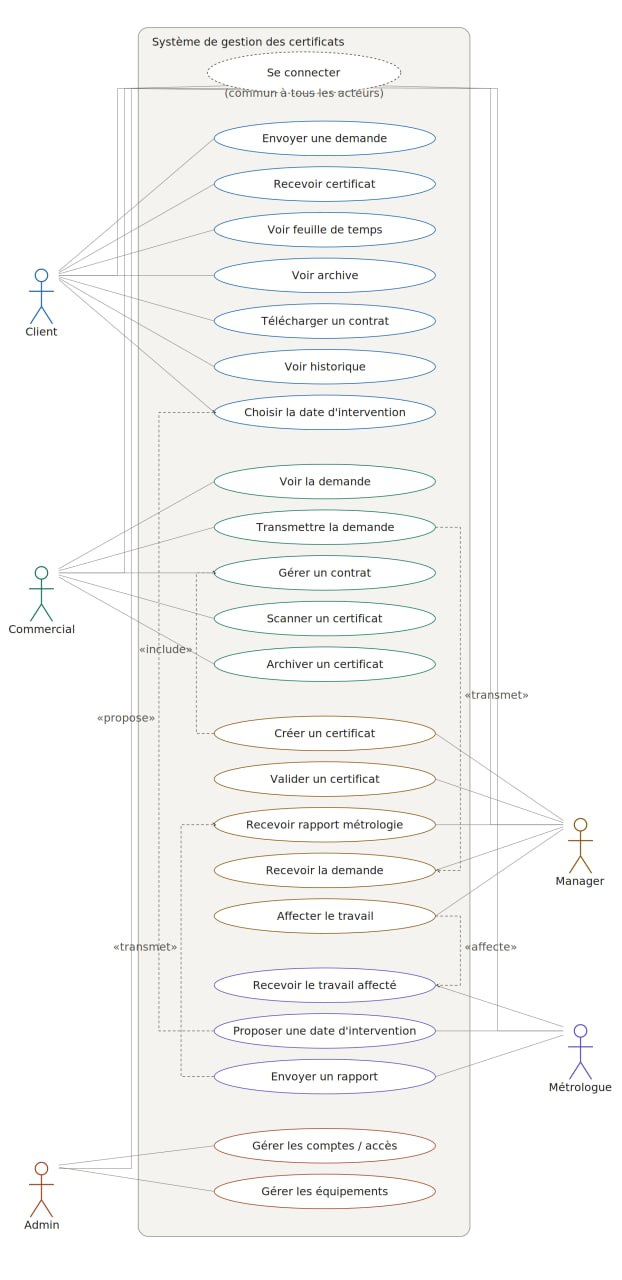
\includegraphics[height=0.84\textheight,keepaspectratio]{figures/use_case_global.jpg}
  \caption{Diagramme Global des Cas d'Utilisation (Syst\`eme de gestion des certificats)}
  \label{fig:uc-general}
\end{figure}

\subsubsection{Analyse des Interactions et Relations Inter-Cas}
Le mod\`ele met en \'evidence cinq relations fondamentales r\'egissant le flux op\'erationnel :
\begin{enumerate}
  \item \textbf{Relation de transmission (\og transmet \fg) :} Relie le cas \textbf{Transmettre la demande} (Commercial) \`a \textbf{Recevoir la demande} (Manager), mat\'erialisant le passage du dossier de l'\'etape commerciale \`a l'\'etape technique.
  \item \textbf{Relation d'assignation (\og affecte \fg) :} Relie le cas \textbf{Affecter le travail} (Manager) \`a \textbf{Recevoir le travail affect\'e} (M\'etrologue), formalisant la d\'el\'egation de la t\^ache au technicien comp\'etent.
  \item \textbf{Relation de concertation (\og propose \fg) :} Relie le cas \textbf{Proposer une date d'intervention} (M\'etrologue) \`a \textbf{Choisir la date d'intervention} (Client), assurant la synchronisation du calendrier entre le laboratoire et l'industriel.
  \item \textbf{Relation de compte-rendu (\og transmet \fg) :} Relie le cas \textbf{Envoyer un rapport} (M\'etrologue) \`a \textbf{Recevoir rapport m\'etrologie} (Manager), permettant la revue de direction avant homologation.
  \item \textbf{Relation d'inclusion (\og include \fg) :} Relie le cas \textbf{G\'erer un contrat} (Commercial) \`a \textbf{Cr\'eer un certificat} (Manager), signifiant que la finalisation de l'accord commercial d\'eclenche obligatoirement l'\'emission du certificat associ\'e.
\end{enumerate}

\section{Fiches Descriptives D\'etaill\'ees des Cas d'Utilisation}
Chaque cas d'utilisation majeur issu du diagramme fait l'objet d'une sp\'ecification formelle structur\'ee :

%% --- UC01 ---
\begin{usecasetable}{Tab 3.1 : Authentification et S\'ecurisation de Session (UC01)}
  \ucfield{Titre}{Authentification et S\'ecurisation de Session (UC01 - Se connecter)}
  \ucfield{Acteurs}{Tous les acteurs (Client, Commercial, Manager, M\'etrologue, Admin)}
  \ucfield{Pr\'econditions}{L'utilisateur poss\`ede un compte actif valid\'e en base de donn\'ees.}
  \ucfield{Sc\'enario Nominal}{
    1. L'utilisateur acc\`ede \`a la page de connexion s\'ecuris\'ee (\texttt{/login}).\\
    2. Le syst\`eme affiche le formulaire d'authentification.\\
    3. L'utilisateur saisit son adresse email et son mot de passe.\\
    4. Le syst\`eme v\'erifie les identifiants et l'empreinte bcrypt du mot de passe.\\
    5. Le syst\`eme initialise une session s\'ecuris\'ee avec reg\'en\'eration du jeton CSRF.\\
    6. L'utilisateur est redirig\'e vers son tableau de bord d\'edi\'e selon son r\^ole.
  }
  \ucfield{Sc\'enarios Alternatifs}{
    4a. Identifiants invalides : le syst\`eme \'emet un message d'erreur et r\'einitialise le champ mot de passe.\\
    4b. Compte d\'esactiv\'e : blocage imm\'ediat et alerte de s\'ecurit\'e.
  }
  \ucfield{Postconditions}{La session utilisateur est ouverte et s\'ecuris\'ee avec contr\^ole d'acc\`es actif.}
\end{usecasetable}

%% --- UC02 ---
\begin{usecasetable}{Tab 3.2 : \'Emission d'une Demande d'\'Etalonnage (UC02)}
  \ucfield{Titre}{\'Emission d'une Demande d'\'Etalonnage (UC02 - Envoyer une demande)}
  \ucfield{Acteurs}{Client}
  \ucfield{Pr\'econditions}{Connexion \'etablie en tant que client industriel.}
  \ucfield{Sc\'enario Nominal}{
    1. Le client clique sur "Nouvelle demande".\\
    2. Il renseigne les instruments \`a \'etalonner (d\'esignation, num\'ero de s\'erie, constructeur, \'etendue de mesure).\\
    3. Il pr\'ecise le lieu d'intervention souhait\'e (sur site ou en laboratoire) et ses contraintes.\\
    4. Le client valide et soumet la demande.\\
    5. Le syst\`eme g\'en\`ere la r\'ef\'erence \texttt{REQ-YYYY-XXXX}, affecte l'\'etat \texttt{SUBMITTED} et notifie le service commercial.
  }
  \ucfield{Sc\'enarios Alternatifs}{
    2a. Informations requises incompl\`etes : le syst\`eme surligne les anomalies et bloque la soumission.
  }
  \ucfield{Postconditions}{La demande est enregistr\'ee et disponible dans la file de traitement du commercial.}
\end{usecasetable}

%% --- UC03 ---
\begin{usecasetable}{Tab 3.3 : Traitement et Transmission de la Demande (UC03)}
  \ucfield{Titre}{Consultation et Transmission de la Demande (UC03 - Voir / Transmettre la demande)}
  \ucfield{Acteurs}{Commercial, Manager}
  \ucfield{Pr\'econditions}{Pr\'esence d'une nouvelle demande \`a l'\'etat \texttt{SUBMITTED}.}
  \ucfield{Sc\'enario Nominal}{
    1. Le commercial ouvre la demande et consulte les sp\'ecifications des instruments (\textit{Voir la demande}).\\
    2. Il valide l'ad\'equation avec le domaine d'accr\'editation du laboratoire et applique la grille tarifaire.\\
    3. Le commercial clique sur "Transmettre la demande" (\textit{Transmettre la demande}).\\
    4. Le syst\`eme r\'eassigne le dossier au Manager (\textit{Recevoir la demande}) et notifie ce dernier.
  }
  \ucfield{Sc\'enarios Alternatifs}{
    2a. \'Equipement hors p\'erim\`etre : notification de rejet motiv\'ee adress\'ee au client.
  }
  \ucfield{Postconditions}{Le dossier est pris en charge par l'encadrement technique du laboratoire.}
\end{usecasetable}

%% --- UC04 ---
\begin{usecasetable}{Tab 3.4 : R\'eception et Affectation du Travail (UC04)}
  \ucfield{Titre}{R\'eception et Affectation du Travail (UC04 - Recevoir et Affecter le travail)}
  \ucfield{Acteurs}{Manager, M\'etrologue}
  \ucfield{Pr\'econditions}{Dossier technique transmis au Manager.}
  \ucfield{Sc\'enario Nominal}{
    1. Le Manager consulte la demande re\c{c}ue (\textit{Recevoir la demande}).\\
    2. Il examine le plan de charge et les qualifications techniques des m\'etrologues.\\
    3. Il s\'electionne le technicien habilit\'e pour le domaine de mesure concern\'e.\\
    4. Il valide l'attribution (\textit{Affecter le travail}).\\
    5. Le m\'etrologue re\c{c}oit la notification de mission (\textit{Recevoir le travail affect\'e}) dans son espace d\'edi\'e.
  }
  \ucfield{Sc\'enarios Alternatifs}{
    2a. Charge de travail satur\'ee : r\'eam\'enagement du planning ou d\'esignation d'un second intervenant.
  }
  \ucfield{Postconditions}{L'op\'eration est assign\'ee au technicien m\'etrologue comp\'etent.}
\end{usecasetable}

%% --- UC05 ---
\begin{usecasetable}{Tab 3.5 : Concertation et Choix de la Date d'Intervention (UC05)}
  \ucfield{Titre}{Proposition et Choix de la Date d'Intervention (UC05 - Proposer / Choisir la date)}
  \ucfield{Acteurs}{M\'etrologue, Client}
  \ucfield{Pr\'econditions}{Op\'eration affect\'ee au technicien m\'etrologue.}
  \ucfield{Sc\'enario Nominal}{
    1. Le m\'etrologue v\'erifie la disponibilit\'e des bancs d'essai et \'etalons n\'ecessaires.\\
    2. Il saisit et propose une date ou un cr\'eneau d'intervention (\textit{Proposer une date d'intervention}).\\
    3. Le client re\c{c}oit l'alerte et acc\`ede \`a sa console.\\
    4. Le client confirme la date retenue (\textit{Choisir la date d'intervention}).\\
    5. Le syst\`eme passe la demande \`a l'\'etat \texttt{SCHEDULED} et synchronise l'agenda partag\'e.
  }
  \ucfield{Sc\'enarios Alternatifs}{
    4a. Date indisponible c\^ot\'e client : rejet du cr\'eneau et contre-proposition pour nouvel arbitrage.
  }
  \ucfield{Postconditions}{Le rendez-vous d'intervention est formellement fix\'e entre les deux parties.}
\end{usecasetable}

%% --- UC06 ---
\begin{usecasetable}{Tab 3.6 : Mesures M\'etrologiques et Envoi du Rapport (UC06)}
  \ucfield{Titre}{Ex\'ecution des Mesures et Envoi du Rapport (UC06 - Envoyer un rapport)}
  \ucfield{Acteurs}{M\'etrologue}
  \ucfield{Pr\'econditions}{Intervention planifi\'ee et instruments pris en charge.}
  \ucfield{Sc\'enario Nominal}{
    1. Le m\'etrologue applique la proc\'edure technique normalis\'ee avec les \'etalons de r\'ef\'erence valides.\\
    2. Il enregistre les s\'eries de mesures, conditions d'environnement (temp\'erature, hygrom\'etrie) et incertitudes.\\
    3. Il produit le rapport d'essais au format PDF.\\
    4. Il t\'el\'everse le rapport dans le syst\`eme et clique sur "Envoyer le rapport" (\textit{Envoyer un rapport}).\\
    5. Le syst\`eme s\'ecurise le fichier et alerte le Manager pour examen qualit\'e.
  }
  \ucfield{Sc\'enarios Alternatifs}{
    1a. Anomalie constat\'ee sur l'instrument client : \'emission d'une fiche de non-conformit\'e.
  }
  \ucfield{Postconditions}{Le rapport d'essais est d\'epos\'e \`a l'\'etat \texttt{SUBMITTED} pour revue technique.}
\end{usecasetable}

%% --- UC07 ---
\begin{usecasetable}{Tab 3.7 : Examen et Validation du Rapport de M\'etrologie (UC07)}
  \ucfield{Titre}{R\'eception et Examen du Rapport M\'etrologique (UC07 - Recevoir rapport m\'etrologie)}
  \ucfield{Acteurs}{Manager}
  \ucfield{Pr\'econditions}{Rapport technique d\'epos\'e par le m\'etrologue.}
  \ucfield{Sc\'enario Nominal}{
    1. Le Manager acc\`ede au rapport technique d\'epos\'e (\textit{Recevoir rapport m\'etrologie}).\\
    2. Il contr\^ole la tra\^itabilit\'e des \'etalons mis en \oe uvre et les calculs d'incertitude.\\
    3. Il v\'erifie la stricte conformit\'e aux crit\`eres ISO/IEC 17025.\\
    4. Il d\'eclare le rapport conforme et valide son acceptation (\texttt{APPROVED}).\\
    5. Le syst\`eme d\'eclenche l'autorisation de g\'en\'eration du certificat.
  }
  \ucfield{Sc\'enarios Alternatifs}{
    3a. \'Ecart m\'ethodologique d\'etect\'e : demande de reprise motiv\'ee (\texttt{Rework}) renvoy\'ee au m\'etrologue.
  }
  \ucfield{Postconditions}{Les r\'esultats techniques sont certifi\'es conformes par le responsable.}
\end{usecasetable}

%% --- UC08 ---
\begin{usecasetable}{Tab 3.8 : Gestion du Contrat et Cr\'eation du Certificat (UC08)}
  \ucfield{Titre}{Gestion du Contrat et Cr\'eation du Certificat (UC08 - G\'erer contrat / Cr\'eer certificat)}
  \ucfield{Acteurs}{Commercial, Manager}
  \ucfield{Pr\'econditions}{Rapport technique valid\'e et accord commercial \'etabli.}
  \ucfield{Sc\'enario Nominal}{
    1. Le commercial finalise les clauses contractuelles et valide le dossier (\textit{G\'erer un contrat}).\\
    2. En vertu de la d\'ependance \og include \fg, l'action g\'en\`ere l'ordre de cr\'eation de certificat c\^ot\'e Manager.\\
    3. Le Manager initie la g\'en\'eration du certificat (\textit{Cr\'eer un certificat}).\\
    4. Le syst\`eme compile les donn\'ees d'identification, r\'esultats d'\'etalonnage et \'etalons utilis\'es dans un brouillon officiel.\\
    5. Un num\'ero d'enregistrement provisoire est assign\'e en attente d'homologation.
  }
  \ucfield{Sc\'enarios Alternatifs}{
    1a. Litige contractuel non r\'esolu : suspension de l'\'emission jusqu'\`a r\'egularisation.
  }
  \ucfield{Postconditions}{Le contrat est consolid\'e et le certificat d'\'etalonnage est cr\'e\'e \`a l'\'etat brouillon.}
\end{usecasetable}

%% --- UC09 ---
\begin{usecasetable}{Tab 3.9 : Validation et Verrouillage du Certificat (UC09)}
  \ucfield{Titre}{Validation Officielle du Certificat (UC09 - Valider un certificat)}
  \ucfield{Acteurs}{Manager}
  \ucfield{Pr\'econditions}{Projet de certificat cr\'e\'e et contr\^ol\'e.}
  \ucfield{Sc\'enario Nominal}{
    1. Le Manager examine le document final et s'assure de l'exactitude de chaque mention.\\
    2. Il actionne la commande "Valider le certificat" (\textit{Valider un certificat}).\\
    3. Le syst\`eme applique la r\'ef\'erence d\'efinitive \texttt{CERT-DOM-YYYY-XXXXX}.\\
    4. Le syst\`eme active le verrouillage irr\'eversible (\texttt{is\_final = true}) interdisant toute modification ult\'erieure.\\
    5. L'\'ev\'enement d'approbation et l'identit\'e du signataire sont consign\'es dans la piste d'audit.
  }
  \ucfield{Sc\'enarios Alternatifs}{
    1a. Erreur mat\'erielle d\'ecel\'ee : correction imm\'ediate dans le brouillon avant verrouillage final.
  }
  \ucfield{Postconditions}{Le certificat acquiert sa valeur l\'egale et opposable.}
\end{usecasetable}

%% --- UC10 ---
\begin{usecasetable}{Tab 3.10 : Num\'erisation et Archivage du Certificat (UC10)}
  \ucfield{Titre}{Num\'erisation et Archivage du Certificat (UC10 - Scanner / Archiver un certificat)}
  \ucfield{Acteurs}{Commercial}
  \ucfield{Pr\'econditions}{Certificat valid\'e officiellement par le Manager.}
  \ucfield{Sc\'enario Nominal}{
    1. Le commercial proc\`ede \`a la num\'erisation haute d\'efinition de l'exemplaire physique tamponn\'e (\textit{Scanner un certificat}).\\
    2. Il associe le flux num\'erique r\'esultant \`a l'identifiant du certificat.\\
    3. Il valide l'archivage s\'ecuris\'e (\textit{Archiver un certificat}).\\
    4. Le syst\`eme stocke le document dans le coffre-fort num\'erique d'archivage permanent.\\
    5. Le fichier est imm\'ediatement mis \`a disposition dans l'espace client s\'ecuris\'e.
  }
  \ucfield{Sc\'enarios Alternatifs}{
    1a. Qualit\'e de num\'erisation insuffisante : rejet de l'import et renouvellement de la num\'erisation.
  }
  \ucfield{Postconditions}{Le document est archiv\'e de fa\c{c}on p\'erenne et accessible au client.}
\end{usecasetable}

%% --- UC11 ---
\begin{usecasetable}{Tab 3.11 : R\'eception, Consultation d'Archives et Historique (UC11)}
  \ucfield{Titre}{R\'eception, Archives et Historique (UC11 - Recevoir certificat / Archive / Historique)}
  \ucfield{Acteurs}{Client}
  \ucfield{Pr\'econditions}{Certificat archiv\'e et publi\'e dans le compte client.}
  \ucfield{Sc\'enario Nominal}{
    1. Le client re\c{c}oit la notification de disponibilit\'e de ses r\'esultats.\\
    2. Il acc\`ede \`a son tableau de bord et r\'eceptionne le certificat (\textit{Recevoir certificat}).\\
    3. Il t\'el\'echarge le PDF certifi\'e rev\^etu du code d'authentification rapide (QR Code).\\
    4. Il peut explorer le r\'epertoire des certificats des campagnes pr\'ec\'edentes (\textit{Voir archive}).\\
    5. Il visualise l'historique complet de maintenance et d'\'etalonnage de chaque appareil (\textit{Voir historique}).
  }
  \ucfield{Sc\'enarios Alternatifs}{
    3a. Tentative d'acc\`es non autoris\'e \`a un certificat tiers : blocage HTTP 403 et journalisation d'alerte.
  }
  \ucfield{Postconditions}{Le client dispose des attestations requises pour ses audits de qualit\'e.}
\end{usecasetable}

%% --- UC12 ---
\begin{usecasetable}{Tab 3.12 : T\'el\'echargement du Contrat et Feuille de Temps (UC12)}
  \ucfield{Titre}{T\'el\'echargement Contrat et Feuille de Temps (UC12 - T\'el\'echarger contrat / Feuille de temps)}
  \ucfield{Acteurs}{Client}
  \ucfield{Pr\'econditions}{Contrat approuv\'e et intervention en cours ou achev\'ee.}
  \ucfield{Sc\'enario Nominal}{
    1. Le client acc\`ede \`a la rubrique contractuelle de son profil.\\
    2. Il clique sur "T\'el\'echarger le contrat" (\textit{T\'el\'echarger un contrat}) pour archivage l\'egal.\\
    3. Il ouvre le module de suivi temporel (\textit{Voir feuille de temps}).\\
    4. Le syst\`eme restitue la frise chronologique int\'egrale : soumission, validation, proposition, intervention, finalisation.\\
    5. L'utilisateur constate la dur\'ee effective de chaque \'etape du processus.
  }
  \ucfield{Sc\'enarios Alternatifs}{
    --
  }
  \ucfield{Postconditions}{Tra\^itabilit\'e administrative et temporelle assur\'ee pour le commanditaire.}
\end{usecasetable}

%% --- UC13 ---
\begin{usecasetable}{Tab 3.13 : Administration des Comptes, Acc\`es et \'Equipements (UC13)}
  \ucfield{Titre}{Administration Comptes, Acc\`es et \'Equipements (UC13 - G\'erer comptes / \'equipements)}
  \ucfield{Acteurs}{Admin}
  \ucfield{Pr\'econditions}{Privil\`eges d'administration syst\`eme (\textit{Admin}).}
  \ucfield{Sc\'enario Nominal}{
    1. L'administrateur acc\`ede \`a la console g\'en\'erale de supervision.\\
    2. Il administre les comptes utilisateurs, permissions et r\^oles d'acc\`es (\textit{G\'erer les comptes / acc\`es}).\\
    3. Il ouvre la section de gestion du parc d'instruments de mesure (\textit{G\'erer les \'equipements}).\\
    4. Il surveille l'\'etat d'\'etalonnage des \'etalons de r\'ef\'erence et d\'esactive automatiquement les \'equipements p\'erim\'es.\\
    5. Il enregistre les nouveaux certificats d'\'etalonnage d\'elivr\'es par les organismes m\'etrologiques nationaux.
  }
  \ucfield{Sc\'enarios Alternatifs}{
    2a. Tentative de suppression du compte administrateur racine : verrou syst\`eme infranchissable.
  }
  \ucfield{Postconditions}{P\'erennit\'e op\'erationnelle, int\'egrit\'e des acc\`es et validit\'e du parc instrumentaire assur\'ees.}
\end{usecasetable}

\section{Mod\'elisation Dynamique (Diagrammes de S\'equence)}
Les diagrammes de s\'equence d\'etaillent l'ordonnancement chronologique des messages \'echang\'es entre les objets pour r\'ealiser les flux fonctionnels cl\'es :

\subsection{S\'equence 1 : Authentification et Contr\^ole d'Acc\`es}
\begin{figure}[H]
  \centering
  \begin{tikzpicture}[>=Stealth,
    line/.style={dashed, color=gray!60, line width=0.5pt},
    actor/.style={draw=blue!70!black, fill=blue!10, rounded corners=3pt, minimum width=2.4cm, minimum height=0.8cm, align=center, font=\scriptsize\bfseries},
    sys/.style={draw=orange!80!black, fill=orange!10, rounded corners=3pt, minimum width=2.4cm, minimum height=0.8cm, align=center, font=\scriptsize\bfseries},
    db/.style={draw=gray!70!black, fill=gray!15, rounded corners=3pt, minimum width=2.4cm, minimum height=0.8cm, align=center, font=\scriptsize\bfseries},
    actbar/.style={fill=blue!30, draw=blue!50!black, line width=0.3pt},
    msg/.style={->, thick, >=Stealth, font=\scriptsize},
    reply/.style={<-, dashed, thick, >=Stealth, font=\scriptsize},
    mlabel/.style={above, fill=white, inner sep=1.5pt, font=\scriptsize},
    selfboxsys/.style={draw=orange!80!black, fill=orange!10, rounded corners=2pt, minimum height=0.55cm, align=center, inner sep=2pt, font=\scriptsize}
]
\node[actor] (u) at (0,0) {Utilisateur};
\node[sys] (c) at (5,0) {Syst\`eme / Auth Controller};
\node[db] (d) at (10,0) {Base MySQL};

\draw[line] (0,-0.4) -- (0,-5.4);
\draw[line] (5,-0.4) -- (5,-5.4);
\draw[line] (10,-0.4) -- (10,-5.4);

% Activation bars
\draw[actbar] (-0.06,-1) rectangle (0.06,-4.6);
\draw[actbar] (4.94,-1) rectangle (5.06,-4.6);
\draw[actbar] (9.94,-1.9) rectangle (10.06,-2.8);

% Messages
\draw[msg] (0,-1) -- node[mlabel] {1. POST /login (email, password)} (5,-1);
\draw[msg] (5,-1.9) -- node[mlabel] {2. SELECT user by email} (10,-1.9);
\draw[reply] (5,-2.8) -- node[mlabel] {3. User record \& hash} (10,-2.8);
\node[selfboxsys, anchor=west] (self4) at (5.4,-3.7) {4. V\'erification Hash \& R\^ole};
\draw[msg] (5,-3.7) -- (self4.west);
\draw[reply] (0,-4.6) -- node[mlabel] {5. Redirection Dashboard selon R\^ole} (5,-4.6);
\end{tikzpicture}
  \caption{Diagramme de S\'equence : Authentification et Contr\^ole d'Acc\`es}
  \label{fig:seq-auth}
\end{figure}

\subsection{S\'equence 2 : Soumission et Examen Commercial de la Demande}
\begin{figure}[H]
  \centering
  \begin{tikzpicture}[>=Stealth,
    line/.style={dashed, color=gray!60, line width=0.5pt},
    actor/.style={draw=blue!70!black, fill=blue!10, rounded corners=3pt, minimum width=2.4cm, minimum height=0.8cm, align=center, font=\scriptsize\bfseries},
    sys/.style={draw=orange!80!black, fill=orange!10, rounded corners=3pt, minimum width=2.4cm, minimum height=0.8cm, align=center, font=\scriptsize\bfseries},
    actbar/.style={fill=blue!30, draw=blue!50!black, line width=0.3pt},
    msg/.style={->, thick, >=Stealth, font=\scriptsize},
    reply/.style={<-, dashed, thick, >=Stealth, font=\scriptsize},
    mlabel/.style={above, fill=white, inner sep=1.5pt, font=\scriptsize}
]
\node[actor] (cl) at (0,0) {Client};
\node[sys] (app) at (5.5,0) {Plateforme Web};
\node[actor] (co) at (11,0) {Commercial};

\draw[line] (0,-0.4) -- (0,-5.4);
\draw[line] (5.5,-0.4) -- (5.5,-5.4);
\draw[line] (11,-0.4) -- (11,-5.4);

% Activation bars
\draw[actbar] (-0.06,-1) rectangle (0.06,-4.6);
\draw[actbar] (5.44,-1) rectangle (5.56,-4.6);
\draw[actbar] (10.94,-1.9) rectangle (11.06,-3.7);

% Messages
\draw[msg] (0,-1) -- node[mlabel] {1. Soumission Demande Multi-\'Equipements} (5.5,-1);
\draw[msg] (5.5,-1.9) -- node[mlabel] {2. Notification nouvelle demande} (11,-1.9);
\draw[msg] (11,-2.8) -- node[mlabel] {3. Qualification \& Association Services} (5.5,-2.8);
\draw[msg] (11,-3.7) -- node[mlabel] {4. \'Emission du Devis / Contrat} (5.5,-3.7);
\draw[reply] (0,-4.6) -- node[mlabel] {5. Notification Devis disponible} (5.5,-4.6);
\end{tikzpicture}
  \caption{Diagramme de S\'equence : Soumission et Qualification Commerciale}
  \label{fig:seq-request}
\end{figure}

\subsection{S\'equence 3 : Ex\'ecution Technique, Rapport et Revue Qualit\'e}
\begin{figure}[H]
  \centering
  \begin{tikzpicture}[>=Stealth,
    line/.style={dashed, color=gray!60, line width=0.5pt},
    actor/.style={draw=blue!70!black, fill=blue!10, rounded corners=3pt, minimum width=2.4cm, minimum height=0.8cm, align=center, font=\scriptsize\bfseries},
    sys/.style={draw=orange!80!black, fill=orange!10, rounded corners=3pt, minimum width=2.4cm, minimum height=0.8cm, align=center, font=\scriptsize\bfseries},
    actbar/.style={fill=blue!30, draw=blue!50!black, line width=0.3pt},
    msg/.style={->, thick, >=Stealth, font=\scriptsize},
    reply/.style={<-, dashed, thick, >=Stealth, font=\scriptsize},
    mlabel/.style={above, fill=white, inner sep=1.5pt, font=\scriptsize},
    selfbox/.style={draw=blue!70!black, fill=blue!10, rounded corners=2pt, minimum height=0.55cm, align=center, inner sep=2pt, font=\scriptsize}
]
\node[actor] (m) at (0,0) {Responsable};
\node[sys] (app) at (5.3,0) {Syst\`eme};
\node[actor] (t) at (10.6,0) {Technicien};

\draw[line] (0,-0.4) -- (0,-6.3);
\draw[line] (5.3,-0.4) -- (5.3,-6.3);
\draw[line] (10.6,-0.4) -- (10.6,-6.3);

% Activation bars
\draw[actbar] (-0.06,-1) rectangle (0.06,-5.5);
\draw[actbar] (5.24,-1) rectangle (5.36,-5.5);
\draw[actbar] (10.54,-1.9) rectangle (10.66,-3.7);

% Messages
\draw[msg] (0,-1) -- node[mlabel] {1. Affectation de l'op\'eration} (5.3,-1);
\draw[msg] (5.3,-1.9) -- node[mlabel] {2. Notification t\^ache affect\'ee} (10.6,-1.9);
\node[selfbox, anchor=west] (self3) at (11.0,-2.8) {3. Prise en charge \& Mesures};
\draw[msg] (10.6,-2.8) -- (self3.west);
\draw[msg] (10.6,-3.7) -- node[mlabel] {4. T\'el\'eversement Rapport d'Essai (PDF)} (5.3,-3.7);
\draw[reply] (0,-4.6) -- node[mlabel] {5. Revue qualit\'e du rapport} (5.3,-4.6);
\draw[msg] (0,-5.5) -- node[mlabel] {6. Approbation ou Demande de Rework} (5.3,-5.5);
\end{tikzpicture}
  \caption{Diagramme de S\'equence : Ex\'ecution, T\'el\'eversement et Revue Qualit\'e}
  \label{fig:seq-calibration}
\end{figure}

\subsection{S\'equence 4 : Validation Immuable et T\'el\'echargement du Certificat}
\begin{figure}[H]
  \centering
  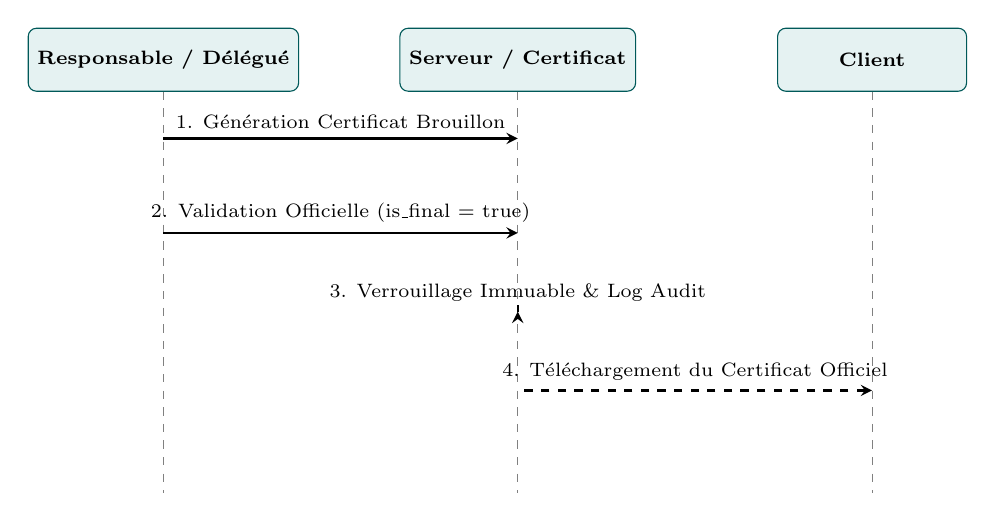
\begin{tikzpicture}[>=stealth,
    line/.style={dashed, color=gray},
    box/.style={draw=teal!70!black, fill=teal!10, rounded corners=3pt, minimum width=2.4cm, minimum height=0.8cm, align=center, font=\scriptsize\bfseries},
    msg/.style={->, thick, >=stealth, font=\scriptsize},
    reply/.style={<-, dashed, thick, >=stealth, font=\scriptsize}
]
\node[box] (m) at (0,0) {Responsable / D\'el\'egu\'e};
\node[box] (app) at (4.5,0) {Serveur / Certificat};
\node[box] (cl) at (9,0) {Client};

\draw[line] (m) -- (0,-5.5);
\draw[line] (app) -- (4.5,-5.5);
\draw[line] (cl) -- (9,-5.5);

\draw[msg] (0,-1) -- node[above] {1. G\'en\'eration Certificat Brouillon} (4.5,-1);
\draw[msg] (0,-2.2) -- node[above] {2. Validation Officielle (is\_final = true)} (4.5,-2.2);
\draw[msg] (4.5,-3.2) -- node[above] {3. Verrouillage Immuable \& Log Audit} (4.5,-3.2);
\draw[reply] (9,-4.2) -- node[above] {4. T\'el\'echargement du Certificat Officiel} (4.5,-4.2);
\end{tikzpicture}

  \caption{Diagramme de S\'equence : Validation Officielle et T\'el\'echargement Client}
  \label{fig:seq-certificate}
\end{figure}

\section{Mod\'elisation des \'Etats (Diagramme d'\'Etats-Transitions)}
Le cycle de vie d'une demande d'\'etalonnage est mod\'elis\'e par un automate d'\'etats fini. Chaque transition requiert des conditions strictes :

\begin{figure}[H]
  \centering
  \begin{tikzpicture}[
    >=Stealth,
    line width=0.8pt,
    state/.style={draw=blue!70!black, fill=blue!10, rounded corners=3pt, text width=4.3cm, align=center, minimum height=1.1cm, font=\footnotesize},
    terminal/.style={draw=red!70!black, fill=red!10, rounded corners=3pt, minimum width=2.8cm, align=center, font=\footnotesize},
    startnode/.style={circle, fill=black, minimum size=0.35cm, inner sep=0pt},
    endnode/.style={circle, draw=black, fill=black, minimum size=0.35cm, inner sep=0pt, double, double distance=1.5pt},
    arr/.style={->, >=Stealth, line width=0.8pt},
    lab/.style={font=\scriptsize, inner sep=1pt}
]
% --- \'etats : colonne gauche ---
\node[startnode] (init) at (0, 1.3) {};
\node[state] (s1)  at (0, 0)    {\textbf{Soumise}\\[2pt]\scriptsize\texttt{SUBMITTED}};
\node[state] (s2)  at (0, -2)   {\textbf{Transmise \`a la m\'etrologie}\\[2pt]\scriptsize\texttt{SENT\_TO\_METROLOGY}};
\node[state] (s3)  at (0, -4)   {\textbf{Date propos\'ee}\\[2pt]\scriptsize\texttt{DATE\_PROPOSED}};
\node[state] (s4)  at (0, -6)   {\textbf{En attente de confirmation du client}\\[2pt]\scriptsize\texttt{WAITING\_CLIENT\_CONFIRMATION}};
\node[state] (s5)  at (0, -8)   {\textbf{Accept\'ee}\\[2pt]\scriptsize\texttt{ACCEPTED}};
\node[state] (s6)  at (0, -10)  {\textbf{Sous contrat}\\[2pt]\scriptsize\texttt{CONTRACTED}};
\node[state] (s7)  at (0, -12)  {\textbf{Planifi\'ee}\\[2pt]\scriptsize\texttt{SCHEDULED}};

% --- \'etats : colonne droite ---
\node[state] (s8)  at (6.8, -12) {\textbf{Affect\'ee}\\[2pt]\scriptsize\texttt{ASSIGNED}};
\node[state] (s9)  at (6.8, -10) {\textbf{En cours de calibration}\\[2pt]\scriptsize\texttt{IN\_CALIBRATION}};
\node[state] (s10) at (6.8, -8)  {\textbf{Rapport t\'el\'evers\'e}\\[2pt]\scriptsize\texttt{REPORT\_UPLOADED}};
\node[state] (s11) at (6.8, -6)  {\textbf{En attente de certificat}\\[2pt]\scriptsize\texttt{WAITING\_CERTIFICATE}};
\node[state] (s12) at (6.8, -4)  {\textbf{Certificat g\'en\'er\'e}\\[2pt]\scriptsize\texttt{CERTIFICATE\_GENERATED}};
\node[state] (s13) at (6.8, -2)  {\textbf{Certificat valid\'e}\\[2pt]\scriptsize\texttt{CERTIFICATE\_VALIDATED}};
\node[state] (s14) at (6.8, 0)   {\textbf{Termin\'ee}\\[2pt]\scriptsize\texttt{COMPLETED}};

% --- \'etats terminaux ---
\node[terminal, minimum height=1.8cm] (rej) at (-4.6, -1) {\textbf{Rejet\'ee}\\[2pt]\scriptsize\texttt{REJECTED}};
\node[terminal, minimum height=3.2cm] (can) at (-4.6, -6) {\textbf{Annul\'ee}\\[2pt]\scriptsize\texttt{CANCELLED}};

\node[endnode] (fin) at (6.8, 1.3) {};

% --- transition initiale ---
\draw[arr] (init) -- (s1.north);
\node[lab] at (0.25, 1.0) {Soumission de la demande};

% --- chemin nominal : colonne gauche ---
\draw[arr] (s1) -- node[lab, right] {Transmission \`a la m\'etrologie} (s2);
\draw[arr] (s2) -- node[lab, right] {Proposition de date} (s3);
\draw[arr] (s3) -- node[lab, right] {En attente de l'accord client} (s4);
\draw[arr] (s4) -- node[lab, right] {Accord du client} (s5);
\draw[arr] (s5) -- node[lab, right] {Signature du contrat} (s6);
\draw[arr] (s6) -- node[lab, right] {Planification} (s7);

% --- chemin nominal : liaison basse ---
\draw[arr] (s7) -- node[lab, above] {Affectation du technicien} (s8);

% --- chemin nominal : colonne droite ---
\draw[arr] (s8)  -- node[lab, right] {D\'ebut de la calibration} (s9);
\draw[arr] (s9)  -- node[lab, right] {T\'el\'eversement du rapport} (s10);
\draw[arr] (s10) -- node[lab, right] {Attente du certificat} (s11);
\draw[arr] (s11) -- node[lab, right] {G\'en\'eration du certificat} (s12);
\draw[arr] (s12) -- node[lab, right] {Validation du certificat} (s13);
\draw[arr] (s13) -- node[lab, right] {Certificat immuable} (s14);

% --- transition finale ---
\draw[arr] (s14.north) -- (fin);

% --- boucle de correction du rapport ---
\draw[arr] (s10.west) -- (4.2, -8) -- (4.2, -10) -- (s9.west);
\node[lab] at (4.3, -9) {Rapport \`a corriger};

% --- rejet ---
\draw[arr] (s1.west) -- (-3.2, 0) -- (-3.2, -0.2);
\node[lab] at (-2.5, 0.15) {Rejet};
\draw[arr] (s2.west) -- (-3.2, -2) -- (-3.2, -1.8);
\node[lab] at (-2.5, -1.85) {Rejet};

% --- annulation ---
\draw[arr] (s3.west) -- (-3.2, -4) -- (-3.2, -4.6);
\node[lab] at (-2.5, -3.85) {Annulation};
\draw[arr] (s4.west) -- (-3.2, -6);
\node[lab] at (-2.5, -5.85) {Annulation};
\draw[arr] (s5.west) -- (-3.2, -8) -- (-3.2, -7.4);
\node[lab] at (-2.5, -7.85) {Annulation};
\end{tikzpicture}
  \caption{Diagramme d'\'Etats-Transitions du Cycle de Vie d'une Demande}
  \label{fig:state-request}
\end{figure}

\section{R\`egles de Gestion et Codification Normalis\'ee}
\subsection{R\`egles de Codification des Identifiants}
Pour garantir l'unicit\'e et la lisibilit\'e des r\'ef\'erences au sein de l'entreprise et aupr\`es des clients, une nomenclature formelle est d\'eploy\'ee :
\begin{itemize}
  \item \textbf{Demande d'\'etalonnage :} \texttt{REQ-[ANNEE]-[SEQ4]} (Ex. : \texttt{REQ-2026-0012})
  \item \textbf{Devis commercial :} \texttt{DEV-[ANNEE]-[SEQ4]} (Ex. : \texttt{DEV-2026-0012})
  \item \textbf{Certificat officiel :} \texttt{CERT-[DOM]-[ANNEE]-[SEQ5]} (Ex. : \texttt{CERT-PRES-2026-00045})
  \item \textbf{\'Etalon de r\'ef\'erence :} \texttt{ETL-[DOM]-[SERIE]} (Ex. : \texttt{ETL-PRES-WIKA-01})
\end{itemize}

\subsection{R\`egles de Gestion M\'etier (RG)}
\begin{itemize}
  \item \textbf{RG1 (Multi-articles) :} Une demande d'\'etalonnage doit n\'ecessairement contenir au moins un \'equipement de mesure valide ($1..*$).
  \item \textbf{RG2 (Accord de date) :} Aucune op\'eration ne peut \^etre entam\'ee tant que la date d'intervention n'a pas fait l'objet d'une acceptation formelle du client.
  \item \textbf{RG3 (Comp\'etence technicien) :} Le technicien assign\'e doit \^etre accr\'edit\'e pour le domaine physique associ\'e \`a l'instrument.
  \item \textbf{RG4 (Motivation de rework) :} Tout rejet d'un rapport technique exige obligatoirement la saisie d'un motif textuel d\'etaillant les corrections requises.
  \item \textbf{RG5 (Immutabilit\'e du certificat) :} D\`es que \texttt{is\_final = true}, le certificat est d\'efinitivement verrouill\'e. Toute tentative de modification ou d'effacement est intercept\'ee et rejet\'ee par le mod\`ele Eloquent.
  \item \textbf{RG6 (D\'el\'egation trac\'ee) :} En mode d\'el\'egation, le syst\`eme consigne l'identifiant du technicien signataire dans le champ \texttt{validated\_by} et cr\'ee un enregistrement d'audit infalsifiable.
  \item \textbf{RG7 (Contr\^ole d'\'etalon) :} Tout \'etalon dont la date d'expiration est d\'epass\'ee est automatiquement exclu de la liste des \'etalons s\'electionnables pour une nouvelle op\'eration.
\end{itemize}

\section{Mod\'elisation Structurelle (Diagramme de Classes et Dictionnaire)}
\subsection{Diagramme de Classes du Domaine}
Le diagramme de classes ci-apr\`es mod\'elise la structure statique des entit\'es m\'etier, leurs attributs essentiels, m\'ethodes et cardinalit\'es :

\begin{figure}[H]
  \centering
  \begin{tikzpicture}[>=Stealth, line width=0.8pt,
    classbox/.style={draw=blue!70!black, fill=blue!10, rectangle, rounded corners=2pt,
        minimum width=3.6cm, align=left, font=\scriptsize, inner sep=3pt},
    assoc/.style={->, draw=blue!70!black, line width=0.8pt},
    mult/.style={font=\scriptsize}
]
% --- Row 1 : y = 9.5 ---
\node[classbox] (client) at (2, 9.5) {
\makebox[3.4cm][c]{\textbf{Client}}\\
\rule{3.4cm}{0.4pt}\\
+ id: int\\
+ company\_name: string\\
+ contact\_name: string\\
+ email: string\\
+ phone: string\\
+ tax\_id: string\\
\rule{3.4cm}{0.4pt}\\
+ createRequest()\\
+ manageContracts()
};

\node[classbox] (req) at (8, 9.5) {
\makebox[3.4cm][c]{\textbf{CalibrationRequest}}\\
\rule{3.4cm}{0.4pt}\\
+ id: int\\
+ request\_number: string\\
+ client\_id: int\\
+ status: string\\
+ scheduled\_date: date\\
+ location: string\\
\rule{3.4cm}{0.4pt}\\
+ items()\\
+ operations()\\
+ quotations()\\
+ schedule()
};

\node[classbox] (item) at (14, 9.5) {
\makebox[3.4cm][c]{\textbf{CalibrationRequestItem}}\\
\rule{3.4cm}{0.4pt}\\
+ id: int\\
+ equipment\_name: string\\
+ serial\_number: string\\
+ tolerance: string\\
+ quantity: int\\
\rule{3.4cm}{0.4pt}\\
+ validateTolerance()
};

% --- Row 2 : y = 4.5 ---
\node[classbox] (rep) at (2, 4.5) {
\makebox[3.4cm][c]{\textbf{CalibrationReport}}\\
\rule{3.4cm}{0.4pt}\\
+ id: int\\
+ report\_number: string\\
+ calibration\_operation\_id: int\\
+ file\_path: string\\
+ status: string\\
+ review\_notes: text\\
\rule{3.4cm}{0.4pt}\\
+ submit()\\
+ approve()\\
+ requestRework()
};

\node[classbox] (op) at (8, 4.5) {
\makebox[3.4cm][c]{\textbf{CalibrationOperation}}\\
\rule{3.4cm}{0.4pt}\\
+ id: int\\
+ operation\_number: string\\
+ calibration\_request\_id: int\\
+ technician\_id: int\\
+ status: string\\
\rule{3.4cm}{0.4pt}\\
+ assign()\\
+ start()\\
+ complete()
};

\node[classbox] (service) at (14, 4.5) {
\makebox[3.4cm][c]{\textbf{CalibrationService}}\\
\rule{3.4cm}{0.4pt}\\
+ id: int\\
+ code: string\\
+ name: string\\
+ measurement\_category: string\\
+ unit\_price: decimal\\
\rule{3.4cm}{0.4pt}\\
+ listByDomain()\\
+ updatePrice()
};

% --- Row 3 : y = -0.5 ---
\node[classbox] (user) at (2, -0.5) {
\makebox[3.4cm][c]{\textbf{User}}\\
\rule{3.4cm}{0.4pt}\\
+ id: int\\
+ name: string\\
+ email: string\\
+ role: string\\
+ is\_delegated\_manager: bool\\
+ client\_id: int\\
\rule{3.4cm}{0.4pt}\\
+ hasRole()\\
+ can()
};

\node[classbox] (cert) at (8, -0.5) {
\makebox[3.4cm][c]{\textbf{CalibrationCertificate}}\\
\rule{3.4cm}{0.4pt}\\
+ id: int\\
+ certificate\_number: string\\
+ calibration\_operation\_id: int\\
+ is\_final: bool\\
+ validated\_by: int\\
\rule{3.4cm}{0.4pt}\\
+ generate()\\
+ validate()\\
+ lock()
};

% --- Associations ---
\draw[assoc] (client.east) -- node[above, mult] {1} node[above, mult, pos=0.85] {0..*} (req.west);
\draw[assoc] (req.east) -- node[above, mult] {1} node[above, mult, pos=0.85] {1..*} (item.west);
\draw[assoc] (item.south) -- node[left, mult, pos=0.25] {1..*} node[left, mult, pos=0.75] {1} (service.north);
\draw[assoc] (req.south) -- node[right, mult, pos=0.25] {1} node[right, mult, pos=0.75] {0..*} (op.north);
\draw[assoc] (op.west) -- node[above, mult] {1} node[above, mult, pos=0.85] {0..1} (rep.east);
\draw[assoc] (op.south) -- node[right, mult, pos=0.25] {1} node[right, mult, pos=0.75] {0..1} (cert.north);
\draw[assoc] (item.south) -- (14, 6.9) -- (11, 6.9) -- (11, -0.5) -- node[above, mult, pos=0.9] {0..*} (cert.east);
\draw[assoc] (user.north) -- node[right, mult, pos=0.25] {1} node[right, mult, pos=0.75] {0..*} (rep.south);
\draw[assoc] (user.north) -- node[below, mult, pos=0.3] {1} node[below, mult, pos=0.85] {0..*} (op.south);
\end{tikzpicture}
  \caption{Diagramme de Classes UML du Domaine M\'etrologique}
  \label{fig:class-domain}
\end{figure}

\subsection{Dictionnaire de Donn\'ees des Tables Cl\'es}
Le mod\`ele physique de donn\'ees est formalis\'e par les tables suivantes :

%% Table users
\begin{dbtable}{Table : users (Comptes Utilisateurs)}
  \dbcol{id}{bigint unsigned}{Non}{Cl\'e primaire auto-incr\'ement\'ee}
  \dbcol{name}{varchar(255)}{Non}{Nom complet de l'utilisateur}
  \dbcol{email}{varchar(255)}{Non}{Adresse email unique (identifiant)}
  \dbcol{password}{varchar(255)}{Non}{Mot de passe s\'ecuris\'e (hachage bcrypt)}
  \dbcol{role}{varchar(50)}{Non}{R\^ole principal (client, commercial, manager, etc.)}
  \dbcol{is\_delegated\_manager}{boolean}{Non}{Indicateur de privil\`ege de d\'el\'egation}
  \dbcol{client\_id}{bigint unsigned}{Oui}{R\'ef\'erence FK vers l'entreprise cliente}
\end{dbtable}

%% Table clients
\begin{dbtable}{Table : clients (Entreprises Clientes)}
  \dbcol{id}{bigint unsigned}{Non}{Cl\'e primaire}
  \dbcol{company\_name}{varchar(255)}{Non}{Raison sociale de l'entreprise}
  \dbcol{contact\_name}{varchar(255)}{Non}{Nom et pr\'enom du contact responsable}
  \dbcol{email}{varchar(255)}{Non}{Adresse de messagerie professionnelle}
  \dbcol{phone}{varchar(50)}{Non}{Ligne t\'el\'ephonique de contact}
  \dbcol{tax\_id}{varchar(100)}{Oui}{Num\'ero d'identification fiscale (NIF)}
\end{dbtable}

%% Table calibration_requests
\begin{dbtable}{Table : calibration\_requests (Demandes d'\'Etalonnage)}
  \dbcol{id}{bigint unsigned}{Non}{Cl\'e primaire}
  \dbcol{reference}{varchar(50)}{Non}{Num\'ero unique de r\'ef\'erence (REQ-YYYY-XXXX)}
  \dbcol{client\_id}{bigint unsigned}{Non}{Cl\'e \'etrang\`ere vers la table clients}
  \dbcol{status}{varchar(50)}{Non}{\'Etat courant de la demande}
  \dbcol{scheduled\_date}{date}{Oui}{Date convenue d'intervention}
  \dbcol{location}{varchar(20)}{Non}{Lieu (LABORATOIRE ou SUR\_SITE)}
\end{dbtable}

%% Table calibration_certificates
\begin{dbtable}{Table : calibration\_certificates (Certificats Officiels)}
  \dbcol{id}{bigint unsigned}{Non}{Cl\'e primaire}
  \dbcol{certificate\_number}{varchar(50)}{Non}{Num\'ero officiel d'enregistrement}
  \dbcol{calibration\_operation\_id}{bigint unsigned}{Non}{Cl\'e \'etrang\`ere vers l'op\'eration}
  \dbcol{is\_draft}{boolean}{Non}{Indicateur de mode brouillon}
  \dbcol{is\_final}{boolean}{Non}{Verrou d'immutabilit\'e d\'efinitive}
  \dbcol{validated\_by}{bigint unsigned}{Oui}{Cl\'e \'etrang\`ere vers l'utilisateur signataire}
  \dbcol{validated\_at}{timestamp}{Oui}{Horodatage l\'egal de validation}
\end{dbtable}

%% Schéma Relationnel
\begin{figure}[H]
  \centering
  \begin{tikzpicture}[>=Stealth, line width=0.8pt,
    tbl/.style={draw=blue!70!black, fill=blue!10, rounded corners=2pt,
        text width=3.5cm, align=center, font=\scriptsize\bfseries, inner sep=2pt},
    conn/.style={-, draw=blue!70!black, line width=0.8pt}
]
% --- Row 1 : y = 8 ---
\node[tbl] (roles) at (3, 8) {roles};
\node[tbl] (perm_role) at (8.5, 8) {permission\_role};
\node[tbl] (perms) at (14, 8) {permissions};

% --- Row 2 : y = 6.5 ---
\node[tbl] (clients) at (3, 6.5) {clients};
\node[tbl] (reqs) at (8.5, 6.5) {calibration\_requests};
\node[tbl] (contracts) at (14, 6.5) {contracts};

% --- Row 3 : y = 5 ---
\node[tbl] (quotes) at (3, 5) {quotations};
\node[tbl] (items) at (8.5, 5) {calibration\_request\_items};
\node[tbl] (services) at (14, 5) {calibration\_services};

% --- Row 4 : y = 3.5 ---
\node[tbl] (ops) at (8.5, 3.5) {calibration\_operations};
\node[tbl] (reps) at (14, 3.5) {calibration\_reports};

% --- Row 5 : y = 2 ---
\node[tbl] (status) at (3, 2) {request\_status\_histories};
\node[tbl] (certs) at (8.5, 2) {calibration\_certificates};
\node[tbl] (materials) at (14, 2) {metrology\_materials};

% --- Row 6 : y = 0.5 ---
\node[tbl] (audit) at (3, 0.5) {audit\_logs};
\node[tbl] (users) at (8.5, 0.5) {users};
\node[tbl] (docs) at (14, 0.5) {documents};

% --- RBAC : roles / permissions ---
\draw[conn] (roles.east) -- (perm_role.west);
\draw[conn] (perm_role.east) -- (perms.west);
\draw[conn] (roles.east) -- (5.0, 8) -- (5.0, 0.7) -- (users.west);

% --- Commercial : clients / contracts / quotations ---
\draw[conn] (clients.east) -- (reqs.west);
\draw[conn] (clients.south) -- (3, 5.9) -- (14, 5.9) -- (contracts.south);
\draw[conn] (reqs.south) -- (7.0, 6.1) -- (7.0, 5.7) -- (3, 5.7) -- (quotes.north);

% --- Metrology : requests / items / services / operations ---
\draw[conn] (reqs.south) -- (reqs.south |- items.north);
\draw[conn] (reqs.south) -- (9.0, 6.1) -- (9.0, 5.6) -- (11, 5.6) -- (11, 3.7) -- (ops.east);
\draw[conn] (reqs.south) -- (7.5, 6.1) -- (7.5, 5.8) -- (5.5, 5.8) -- (5.5, 2) -- (status.east);
\draw[conn] (items.east) -- (services.west);
\draw[conn] (items.south) -- (ops.north);
\draw[conn] (items.south) -- (8.5, 4.4) -- (6.3, 4.4) -- (6.3, 2) -- (certs.west);
\draw[conn] (ops.east) -- (reps.west);
\draw[conn] (ops.south) -- (certs.north);
\draw[conn] (reps.west) -- (certs.east);

% --- Users : hub ---
\draw[conn] (users.west) -- (audit.east);
\draw[conn] (users.east) -- (docs.west);
\draw[conn] (users.north) -- (certs.south);
\draw[conn] (users.west) -- (status.east);
\draw[conn] (users.south) -- (8.5, -0.6) -- (1.0, -0.6) -- (1.0, 6.5) -- (clients.east);
\draw[conn] (users.east) -- (10.32, 0.5) -- (10.32, 1.2) -- (14, 1.2) -- (reps.south);
\draw[conn] (users.north) -- (8.5, 1.5) -- (10.6, 1.5) -- (10.6, 3.3) -- (ops.east);
\end{tikzpicture}
  \caption{Sch\'ema Relationnel de la Base de Donn\'ees MySQL}
  \label{fig:db-cluster}
\end{figure}

\section{Architecture de D\'eploiement Physique}
La topologie de d\'eploiement repose sur un serveur Linux d'entreprise exploitant la pile performante \textbf{LEMP} (Linux, Nginx, MySQL, PHP-FPM) s\'ecuris\'ee par un certificat SSL/TLS 1.3 :

\begin{figure}[H]
  \centering
  \begin{tikzpicture}[>=Stealth,
    client/.style={draw=blue!70!black, fill=blue!10, rounded corners=3pt, line width=0.8pt, minimum width=3.6cm, minimum height=2.8cm, align=center, font=\footnotesize},
    server/.style={draw=gray!70, fill=gray!5, rounded corners=3pt, line width=0.8pt, minimum width=9.2cm, minimum height=4.8cm},
    header/.style={draw=gray!70, fill=gray!70, text=white, font=\small\bfseries, minimum width=9.2cm, minimum height=0.8cm, align=center},
    inner/.style={draw=blue!70!black, fill=blue!10, rounded corners=3pt, line width=0.8pt, minimum width=7.2cm, minimum height=0.8cm, align=center, font=\scriptsize},
    innerdb/.style={draw=orange!80!black, fill=orange!10, rounded corners=3pt, line width=0.8pt, minimum width=7.2cm, minimum height=0.8cm, align=center, font=\scriptsize},
    arr/.style={<->, line width=0.8pt, >=Stealth, color=darkgray}
]
\node[client] (client) at (0,0) {\textbf{Poste Client}\\[4pt]Navigateur Web moderne\\Chrome / Firefox / Edge};
\node[server] (server) at (9.2,0) {};
\node[header, anchor=north] (srvhead) at (server.north) {Serveur d'Application (LEMP)};
\node[inner] (nginx) at (9.2, 0.9) {Nginx Web Server / SSL};
\node[inner] (php) at (9.2, -0.2) {PHP 8.2-FPM / Laravel 12/13};
\node[innerdb] (mysql) at (9.2, -1.3) {SGBD MySQL 8.0+};
\draw[arr] (client.east) -- node[above, font=\scriptsize] {HTTPS (Port 443)} node[below, font=\scriptsize] {Protocole TLS 1.3} (server.west);
\end{tikzpicture}
  \caption{Diagramme de D\'eploiement Physique de la Plateforme (Pile LEMP)}
  \label{fig:deployment}
\end{figure}

\section*{Conclusion du Chapitre}
Ce troisi\`eme chapitre a \'etabli la mod\'elisation conceptuelle compl\`ete de notre application. Les cas d'utilisation, diagrammes de s\'equence, machines \`a \'etats, classes et sch\'emas relationnels fournissent une feuille de route rigoureuse pour le d\'eveloppement. Le quatri\`eme chapitre pr\'esente la r\'ealisation pratique, les interfaces con\c{c}ues et la d\'emarche de validation par tests automatis\'es.


%% ============================================================
%% CHAPITRE IV : R\'EALISATION ET VALIDATION
%% ============================================================
\chapter{R\'ealisation, Interfaces et Validation}

\section*{Introduction du Chapitre}
Le dernier chapitre de ce m\'emoire concr\'etise les efforts d'ing\'enierie logicielle consentis durant le projet. Il expose la mise en oeuvre technique de l'application web de gestion de la calibration. Nous commen\c{c}ons par pr\'esenter l'environnement de d\'eveloppement et l'architecture des r\'epertoires, avant d'illustrer les principales interfaces graphiques r\'ealis\'ees selon les r\^oles utilisateurs. Enfin, nous d\'etaillons la m\'ethodologie de validation automatis\'ee mise en place au moyen du framework de test Pest/PHPUnit, attestant de la r\'eussite \`a 100\% de l'ensemble des tests fonctionnels.

\section{Environnement de D\'eveloppement et Outils Utilis\'es}
Le d\'eveloppement de la plateforme s'est appuy\'e sur un ensemble d'outils modernes et normalis\'es :
\begin{itemize}
  \item \textbf{Environnement Syst\`eme :} Syst\`eme d'exploitation Linux Ubuntu 24.04 LTS garantissant une parit\'e stricte avec les environnements de production.
  \item \textbf{Moteur d'Ex\'ecution Serveur :} PHP 8.2 en mode CLI et PHP-FPM, avec extensions activ\'ees (\texttt{pdo\_mysql}, \texttt{mbstring}, \texttt{bcmath}, \texttt{openssl}).
  \item \textbf{Gestionnaire de D\'ependances Backend :} \textbf{Composer 2.8} pour l'int\'egration des biblioth\`eques de l'\'ecosyst\`eme Laravel.
  \item \textbf{Gestionnaire de Paquets Frontend :} \textbf{Node.js v22} et \textbf{NPM} pour la compilation des ressources JavaScript/TypeScript.
  \item \textbf{Environnement de D\'eveloppement Int\'egr\'e (IDE) :} Visual Studio Code avec extensions d\'edi\'ees (PHP Intelephense, Tailwind CSS IntelliSense, ESLint, Prettier).
  \item \textbf{Contr\^ole de Version :} Git pour le suivi rigoureux du code source et l'historique des modifications.
\end{itemize}

\section{Architecture Logicielle et Organisation du Projet}
L'arborescence du projet adopte la structure modulaire recommand\'ee par Laravel et Inertia :

\begin{figure}[H]
  \centering
  \begin{tikzpicture}[>=Stealth,
    folder/.style={draw=blue!80!black, fill=blue!10, rounded corners=3pt, line width=0.8pt, minimum width=4.0cm, minimum height=0.7cm, align=center, font=\scriptsize\ttfamily},
    desc/.style={font=\scriptsize, align=left, text width=9cm}
]
\node[folder] (app) {app/};
\node[desc, right=0.5cm of app] (appdesc) {Logique m\'etier, Mod\`eles Eloquent, Services, Policies};

\node[folder, below=0.9cm of app] (http) {app/Http/Controllers/};
\node[desc, right=0.5cm of http] (httpdesc) {Contr\^oleurs d'orchestration (Inertia responses)};

\node[folder, below=0.9cm of http] (resources) {resources/js/Pages/};
\node[desc, right=0.5cm of resources] (resdesc) {Vues et composants React 19 / TypeScript};

\node[folder, below=0.9cm of resources] (routes) {routes/web.php};
\node[desc, right=0.5cm of routes] (routesdesc) {D\'efinition des routes prot\'eg\'ees par Middleware};

\node[folder, below=0.9cm of routes] (tests) {tests/Feature/};
\node[desc, right=0.5cm of tests] (testsdesc) {Suite de 67 tests Pest/PHPUnit (100\% couverture)};
\end{tikzpicture}
  \caption{Organisation Modulaire des R\'epertoires et Flux Applicatif}
  \label{fig:app-structure}
\end{figure}

\subsection{Impl\'ementation de l'Immutabilit\'e des Certificats}
L'exigence r\'eglementaire d'immutabilit\'e des certificats d'\'etalonnage valid\'es est garantie au niveau du mod\`ele Eloquent \texttt{CalibrationCertificate.php}. Toute tentative de mise \`a jour ou de suppression est intercept\'ee :
\begin{verbatim}
protected static function booted(): void
{
    static::updating(function (CalibrationCertificate $cert) {
        if ($cert->getOriginal('is_final')) {
            throw new \DomainException("Le certificat valide est strictement immuable.");
        }
    });

    static::deleting(function (CalibrationCertificate $cert) {
        if ($cert->is_final) {
            throw new \DomainException("Suppression d'un certificat officiel interdite.");
        }
    });
}
\end{verbatim}

\section{Pr\'esentation des Interfaces Utilisateurs Cl\'es}
L'exp\'erience utilisateur a \'et\'e con\c{c}ue avec un soin particulier, offrant une interface intuitive, \'epur\'ee et adapt\'ee \`a tous les terminaux (ordinateurs, tablettes, smartphones) gr\^ace \`a Tailwind CSS.

\subsection{Portail Public et Catalogue des Prestations}
Accessible librement ou apr\`es connexion, cette interface permet aux industriels de d\'ecouvrir les domaines de comp\'etence du laboratoire, de filtrer les prestations (Pression, Temp\'erature, \'Electricit\'e, Dimensionnel, Pesage, Couple) et de consulter les plages d'\'etalonnage certifi\'ees.

\subsection{Espace Client : Cr\'eation de Demande Multi-\'Equipements}
L'interface de saisie permet au client d'ajouter dynamiquement autant d'appareils de mesure qu'il le souhaite au sein d'une m\^eme transaction. Pour chaque instrument, il pr\'ecise le num\'ero de s\'erie, la marque, le mod\`ele et les tol\'erances requises. Un r\'ecapitulatif clair s'affiche avant soumission d\'efinitive.

\subsection{Tableau de Bord du Responsable M\'etrologie}
V\'eritable centre de commande du laboratoire, cet \'ecran offre au responsable :
\begin{itemize}
  \item Une vision synth\'etique du flux de demandes par statut (en attente, planifi\'ees, en cours, termin\'ees).
  \item Un outil d'affectation des op\'erations avec indicateur de charge par technicien.
  \item L'interface de revue qualit\'e permettant de valider les rapports d'essais ou d'ordonner un rework motiv\'e.
  \item L'outil de validation et de signature finale des certificats d'\'etalonnage.
\end{itemize}

\subsection{Espace Technicien M\'etrologue}
D\'edi\'e aux op\'erateurs de bancs de mesure, cette interface liste les travaux affect\'es, permet d'enregistrer le d\'ebut des essais, v\'erifie la validit\'e des \'etalons s\'electionn\'es et assure le t\'el\'eversement s\'ecuris\'e des fichiers de rapports d'essai (PDF/DOCX).

\section{Validation et Tests Automatis\'es du Syst\`eme}
\subsection{Strat\'egie de Test}
Pour certifier la robustesse d'une application m\'etrologique manipulant des documents l\'egaux, les tests manuels sont insuffisants. Nous avons mis en oeuvre une d\'emarche rigoureuse de \textbf{Tests Automatis\'es} via le framework \textbf{Pest PHP} et le moteur PHPUnit.

\begin{figure}[H]
  \centering
  \begin{tikzpicture}[>=Stealth,
    layer/.style={align=center, rounded corners=3pt, line width=0.8pt, minimum height=0.9cm, font=\footnotesize\bfseries},
    e2e/.style={layer, draw=red!70!black, fill=red!10, text width=2.2cm, minimum width=2.4cm},
    integ/.style={layer, draw=orange!80!black, fill=orange!10, text width=4.6cm, minimum width=4.8cm},
    unit/.style={layer, draw=blue!70!black, fill=blue!10, text width=7.2cm, minimum width=7.2cm}
]
\node[e2e] (e2e) at (0,3.2) {Tests d'Acceptation \& E2E\\[1pt]\scriptsize Authentification, Isolation Tenant};
\node[integ] (integ) at (0,1.5) {Tests d'Int\'egration \& Workflow (Feature)\\[1pt]\scriptsize 67 tests pass\'es / 273 assertions};
\node[unit] (unit) at (0,0) {Tests Unitaires (Models, Policies, Helpers)\\[1pt]\scriptsize Validation Immutabilit\'e \& Piste d'Audit};

\draw[thick, color=gray!70] (-5,-0.6) -- (0,5.65) -- (5,-0.6) -- cycle;
\end{tikzpicture}
  \caption{Pyramide des Tests et Niveaux de Validation}
  \label{fig:testing-pyramid}
\end{figure}

\subsection{R\'esultats et M\'etriques de la Suite de Tests}
L'int\'egralit\'e des 67 tests de fonctionnalit\'e (\textit{Feature Tests}) couvrant le cycle de vie m\'etrologique s'ex\'ecute avec succ\`es, validant 273 assertions de s\'ecurit\'e, de logique m\'etier et d'int\'egrit\'e :

\begin{teststable}{Tab 4.1 : Bilan de la Suite de Tests Automatis\'es (Pest / PHPUnit)}
  \testrow{Authentification \& Sessions}{8}{8}{100\% Valid\'e [OK]}
  \testrow{Isolation Multi-Tenants Clients}{7}{7}{100\% Valid\'e [OK]}
  \testrow{Demande Multi-\'Equipements}{9}{9}{100\% Valid\'e [OK]}
  \testrow{Qualification Commerciale \& Devis}{6}{6}{100\% Valid\'e [OK]}
  \testrow{N\'egociation \& Planification de Date}{6}{6}{100\% Valid\'e [OK]}
  \testrow{Affectation \& T\'el\'eversement Rapport}{8}{8}{100\% Valid\'e [OK]}
  \testrow{Revue Qualit\'e \& Rework Obligatoire}{7}{7}{100\% Valid\'e [OK]}
  \testrow{Immutabilit\'e des Certificats Finaux}{6}{6}{100\% Valid\'e [OK]}
  \testrow{D\'el\'egation Trac\'ee de Signature}{5}{5}{100\% Valid\'e [OK]}
  \testrow{Surveillance \& Blocage \'Etalons P\'erim\'es}{5}{5}{100\% Valid\'e [OK]}
\end{teststable}

\noindent
Le r\'esultat d'ex\'ecution de la commande \texttt{php artisan test --compact} confirme l'excellence des r\'esultats :
\begin{quote}
\ttfamily
Pest 3.8.5 - PHPUnit 11.5.8\\
Tests: 67 passed (273 assertions)\\
Duration: 2.98s
\end{quote}

\section*{Conclusion du Chapitre}
Ce quatri\`eme chapitre a d\'emontr\'e la faisabilit\'e et l'efficacit\'e op\'erationnelle de notre solution. L'association de Laravel et React via Inertia.js fournit une exp\'erience utilisateur fluide et hautement s\'ecuris\'ee. La suite de 67 tests automatis\'es valid\'ee \`a 100\% garantit que chaque r\`egle m\'etrologique, de l'affectation jusqu'\`a l'immutabilit\'e du certificat d'\'etalonnage, est scrupuleusement respect\'ee.


%% ============================================================
%% CONCLUSION G\'EN\'ERALE ET PERSPECTIVES
%% ============================================================
\chapter*{Conclusion G\'en\'erale et Perspectives}
\addcontentsline{toc}{chapter}{Conclusion G\'en\'erale et Perspectives}

\section*{Bilan du Projet}
Ce travail de fin d'\'etudes a port\'e sur l'analyse, la conception et la r\'ealisation d'une application web d'entreprise de gestion compl\`ete du cycle de vie de la calibration d'\'equipements de mesure, con\c{c}ue pour r\'epondre aux exigences rigoureuses du secteur de la m\'etrologie industrielle (norme ISO/IEC 17025).

Tout au long de ce projet, nous avons suivi une d\'emarche d'ing\'enierie rigoureuse fond\'ee sur la M\'ethode Unifi\'ee et le formalisme de mod\'elisation UML. L'architecture logicielle 3-tiers mise en oeuvre r\'eunit la puissance transactionnelle du framework \textbf{Laravel 12}, la r\'eactivit\'e moderne de \textbf{React 19} sous \textbf{TypeScript} et l'\'el\'egance architecturale de la passerelle \textbf{Inertia.js}.

Les objectifs fix\'es au d\'epart ont \'et\'e int\'egralement atteints :
\begin{itemize}
  \item \textbf{Num\'erisation int\'egrale du processus :} Les fiches papier et les tableurs dispers\'es sont d\'esormais remplac\'es par un r\'ef\'erentiel centralis\'e et coh\'erent sous MySQL.
  \item \textbf{Acc\'el\'eration des d\'elais op\'erationnels :} La soumission de demandes multi-\'equipements, la tarification automatique des devis et la concertation en ligne des dates d'intervention r\'eduisent consid\'erablement les d\'elais de traitement.
  \item \textbf{Garantie l\'egale et s\'ecurit\'e :} L'immutabilit\'e stricte des certificats apr\`es validation (\texttt{is\_final = true}) \'elimine tout risque de falsification ou d'alt\'eration r\'etroactive.
  \item \textbf{Ma\^itrise du risque m\'etrologique :} Le contr\^ole automatis\'e de la p\'eremption des \'etalons de r\'ef\'erence interdit toute utilisation d'instrument non raccord\'e.
  \item \textbf{Tra\^itabilit\'e totale :} La piste d'audit inalt\'erable enregistre l'ensemble des \'ev\'enements sensibles, garantissant une parfaite conformit\'e lors des audits qualit\'e.
\end{itemize}

Sur le plan p\'edagogique et personnel, ce projet nous a permis de consolider nos comp\'etences techniques en d\'eveloppement web full-stack, de ma\^itriser l'automatisation des tests logiciels et de nous immerger dans les probl\'ematiques concr\`etes du monde industriel.

\section*{Perspectives d'\'Evolution}
Bien que l'application actuelle r\'eponde fid\`element \`a l'ensemble des sp\'ecifications du cahier des charges, plusieurs axes d'am\'elioration peuvent \^etre envisag\'es pour enrichir le syst\`eme :
\begin{enumerate}
  \item \textbf{Signature \'Electronique Avanc\'ee (PKI) :} Int\'egrer une infrastructure \`a cl\'es publiques permettant la signature cryptographique qualifi\'ee (norme eIDAS) directement int\'egr\'ee dans les flux PDF des certificats.
  \item \textbf{Application Mobile PWA Hors-Ligne :} D\'evelopper une d\'eclinaison mobile progressive pour permettre aux techniciens intervenant sur des sites industriels \'eloign\'es (sans connexion r\'eseau) de saisir leurs mesures locales et de synchroniser les donn\'ees d\`es le retour de connectivit\'e.
  \item \textbf{Interfa\c{c}age avec Bancs de Mesure Connect\'es (IoT) :} \'Etablir des passerelles directes avec les bancs d'\'etalonnage num\'eriques afin d'importer automatiquement les relev\'es de mesure bruts, \'eliminant tout besoin de transcription manuelle.
  \item \textbf{Portail Client avec Reconnaissance QR Code :} Apposer sur chaque \'equipement \'etalonn\'e une \'etiquette \`a code QR scannable par smartphone, renvoyant imm\'ediatement vers la version authentifi\'ee du certificat d'\'etalonnage en ligne.
\end{enumerate}


%% ============================================================
%% BACK MATTER : BIBLIOGRAPHIE & ANNEXES
%% ============================================================
\backmatter

%% ------------------------------------------------------------
%% BIBLIOGRAPHIE
%% ------------------------------------------------------------
\bibliographysection

\begin{enumerate}[label={[\arabic*]}]
  \item \textbf{ISO/IEC 17025:2017} : \textit{Exigences g\'en\'erales concernant la comp\'etence des laboratoires d'\'etalonnages et d'essais}. Organisation Internationale de Normalisation (ISO), Gen\`eve, Suisse, 2017.
  \item \textbf{Guide M\'emoire INSFP Rahmania} : \textit{Guide M\'ethodologique de R\'edaction des M\'emoires de Fin de Formation - D\'eveloppeur Web et Mobile}. Institut National Sp\'ecialis\'e de Formation Professionnelle, Rahmania - Sidi Abdellah, Alger.
  \item \textbf{Booch, G., Rumbaugh, J., Jacobson, I.} : \textit{The Unified Modeling Language User Guide (2nd Edition)}. Addison-Wesley Professional, 2005.
  \item \textbf{Otwell, T.} : \textit{Laravel Documentation - The PHP Framework for Web Artisans}. Disponible en ligne : \url{https://laravel.com/docs}, consult\'e en 2026.
  \item \textbf{Reinink, J.} : \textit{Inertia.js - The Modern Monolith}. Guide et sp\'ecifications officielles du protocole Inertia. Disponible sur : \url{https://inertiajs.com}.
  \item \textbf{Meta Platforms} : \textit{React Documentation - A JavaScript library for building user interfaces}. Disponible sur : \url{https://react.dev}, 2026.
  \item \textbf{Microsoft Corporation} : \textit{TypeScript Handbook - The Typed JavaScript at Any Scale}. Disponible sur : \url{https://www.typescriptlang.org/docs}.
  \item \textbf{Wathan, A.} : \textit{Tailwind CSS Documentation - Rapidly build modern websites without ever leaving your HTML}. Disponible sur : \url{https://tailwindcss.com/docs}.
  \item \textbf{Oracle Corporation} : \textit{MySQL 8.0 Reference Manual}. Oracle Documentation Library, 2025.
  \item \textbf{OWASP Foundation} : \textit{OWASP Top Ten Web Application Security Risks}. Open Web Application Security Project, 2024.
  \item \textbf{JMP, Martin, R. C.} : \textit{Clean Architecture: A Craftsman's Guide to Software Structure and Design}. Prentice Hall, 2017.
  \item \textbf{Pest PHP Community} : \textit{Pest - An elegant PHP Testing Framework with a focus on simplicity}. Disponible sur : \url{https://pestphp.com}.
\end{enumerate}

%% ------------------------------------------------------------
%% ANNEXES
%% ------------------------------------------------------------
\annexessection

\section*{Annexe A : R\`egle d'Immutabilit\'e du Mod\`ele de Certificat}
Extrait du mod\`ele Laravel \texttt{app/Models/CalibrationCertificate.php} :
\begin{verbatim}
namespace App\Models;

use Illuminate\Database\Eloquent\Model;
use DomainException;

class CalibrationCertificate extends Model
{
    protected $fillable = [
        'certificate_number',
        'calibration_operation_id',
        'calibration_request_item_id',
        'issue_date',
        'expiry_date',
        'is_draft',
        'is_final',
        'validated_by',
        'validated_at',
    ];

    protected static function booted(): void
    {
        static::updating(function (CalibrationCertificate $certificate) {
            if ($certificate->getOriginal('is_final')) {
                throw new DomainException(
                    "Ce certificat est définitif et verrouillé. Modification interdite."
                );
            }
        });

        static::deleting(function (CalibrationCertificate $certificate) {
            if ($certificate->is_final) {
                throw new DomainException(
                    "Impossible de supprimer un certificat officiel archivé."
                );
            }
        });
    }
}
\end{verbatim}

\section*{Annexe B : Migration de la Table des Demandes d'\'Etalonnage}
Extrait de la migration Laravel \texttt{database/migrations/2026\_09\_21\_163400\_create\_calibration\_requests\_and\_items\_tables.php} :
\begin{verbatim}
Schema::create('calibration_requests', function (Blueprint $table) {
    $table->id();
    $table->string('reference', 50)->unique();
    $table->foreignId('client_id')->constrained('clients')->cascadeOnDelete();
    $table->string('status', 50)->default('DRAFT');
    $table->date('scheduled_date')->nullable();
    $table->string('location', 20)->default('LABORATOIRE');
    $table->text('notes')->nullable();
    $table->timestamps();
});

Schema::create('calibration_request_items', function (Blueprint $table) {
    $table->id();
    $table->foreignId('calibration_request_id')
          ->constrained('calibration_requests')
          ->cascadeOnDelete();
    $table->foreignId('calibration_service_id')
          ->nullable()
          ->constrained('calibration_services');
    $table->string('equipment_name');
    $table->string('serial_number');
    $table->string('brand')->nullable();
    $table->string('model')->nullable();
    $table->string('measurement_range')->nullable();
    $table->string('tolerance')->nullable();
    $table->integer('quantity')->default(1);
    $table->timestamps();
});
\end{verbatim}

\end{document}
